\documentclass[12pt, letterpaper]{article}
\usepackage[
    backend=biber,
    style=alphabetic,
]{biblatex} 
\usepackage{graphicx}
\usepackage{enumitem}
\usepackage{pdfpages}
\usepackage{listings, listings-rust}
\graphicspath{{diagrams/}}
\addbibresource{sources.bib}

\title{
    \Huge \textbf{Software-Implemented Fault Tolerance}
}
\author{Filip Ďuriš}

\definecolor{codegreen}{rgb}{0,0.6,0}
\definecolor{codegray}{rgb}{0.5,0.5,0.5}
\definecolor{codepurple}{rgb}{0.58,0,0.82}
\definecolor{backcolour}{rgb}{0.95,0.95,0.95}

\lstdefinestyle{mystyle}{
    backgroundcolor=\color{backcolour},   
    commentstyle=\color{codegreen},
    keywordstyle=\color{magenta},
    numberstyle=\tiny\color{codegray},
    stringstyle=\color{codepurple},
    basicstyle=\ttfamily\footnotesize,
    breakatwhitespace=false,         
    breaklines=true,                 
    captionpos=b,                    
    keepspaces=true,                 
    numbers=left,                    
    numbersep=5pt,                  
    showspaces=false,                
    showstringspaces=false,
    showtabs=false,                  
    tabsize=2
}

\lstset{style=mystyle}

\begin{document}

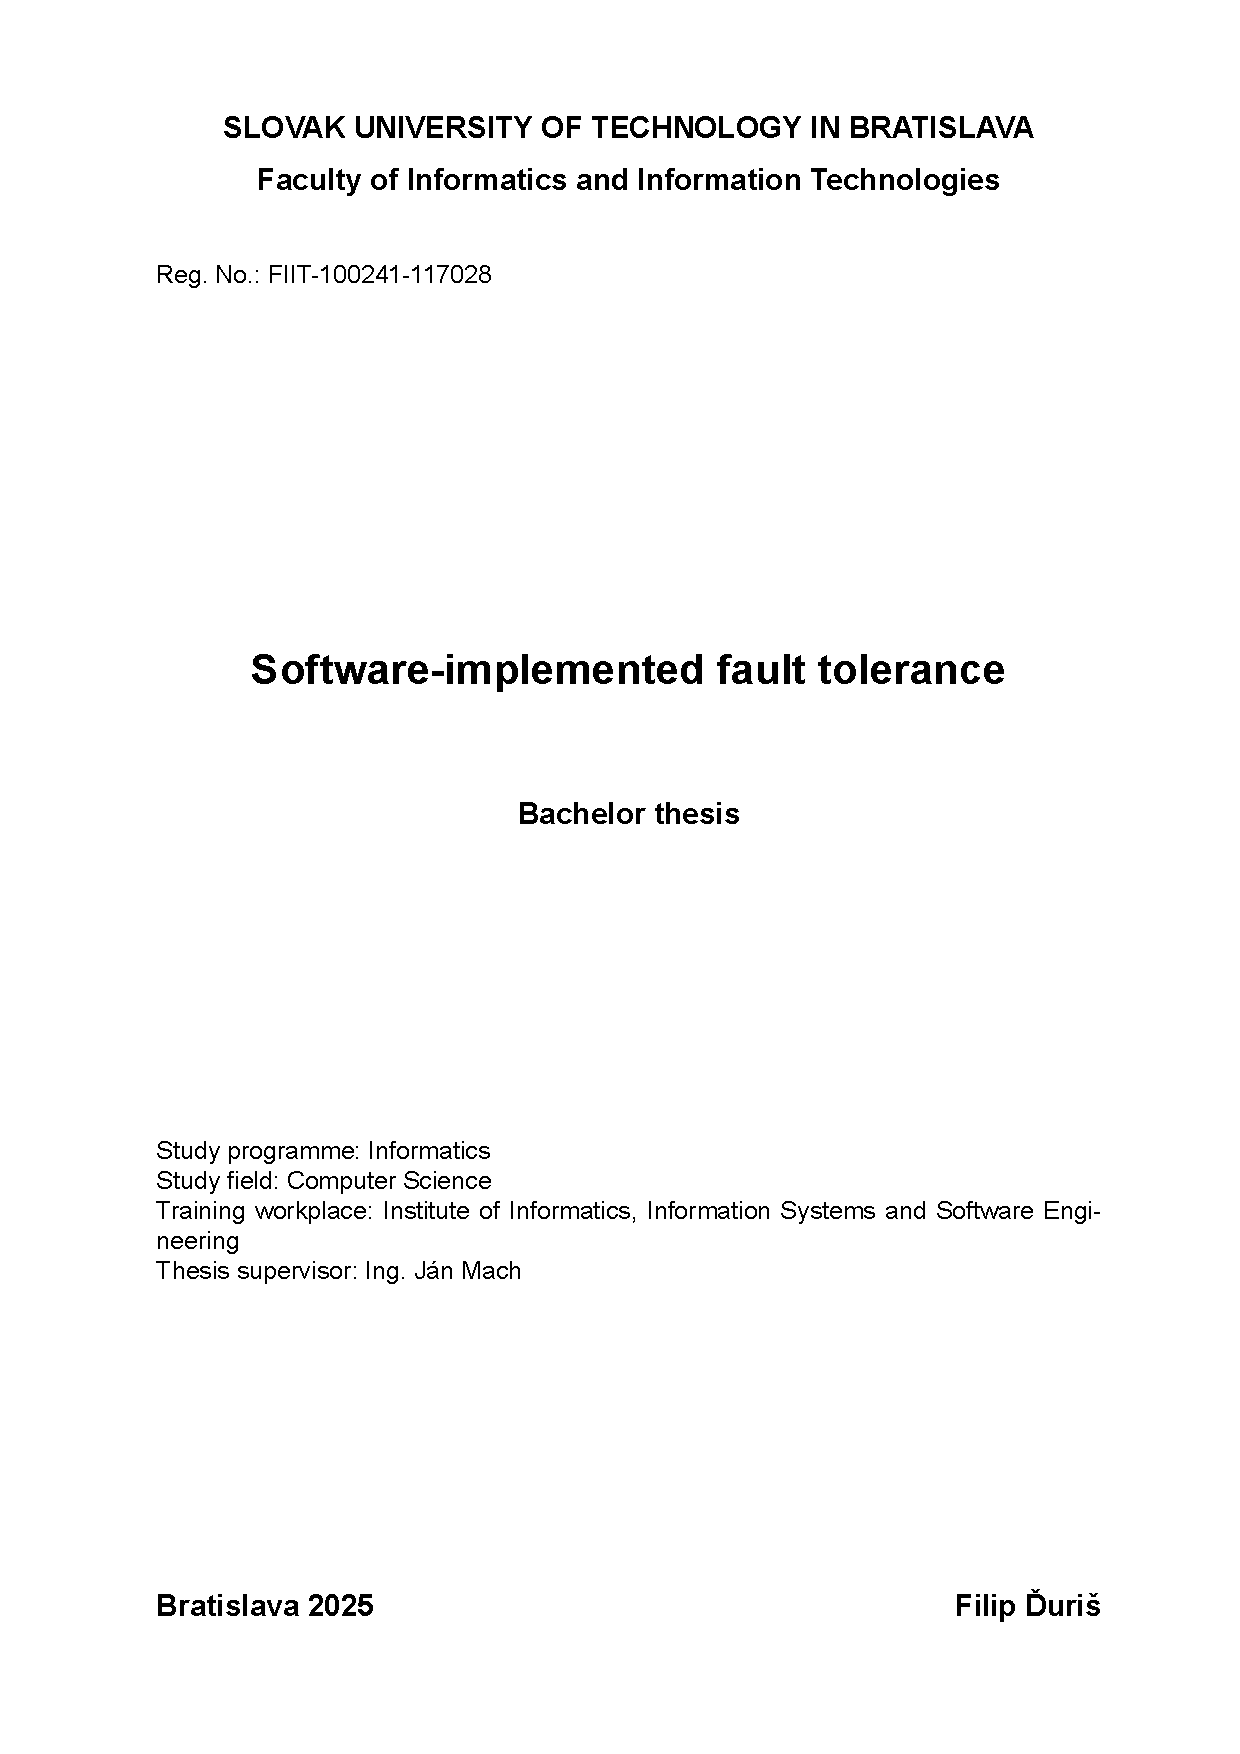
\includepdf[pages={1}]{front_page.pdf}

% \maketitle

\newpage

\begin{abstract}
With the increasing demand for high-performance embedded software comes the inevitable, difficult task of ensuring fault-free functioning of ever-more complex systems. The increased complexity, both in terms of hardware components and software features, increases the number of failure points where errors can manifest.

Errors can be caused by both external factors beyond our control such as radiation in space, but also as a result of human error while designing the software. Due to the incredibly complex nature of this problem, it is unlikely that we will be designing completely error-free software and hardware in the near future. This simple fact makes fault-tolerance an important aspect of software design, especially when designing critical systems whose failure could endanger human life. However, as with most things, fault-tolerance and reliability is a trade-off, which usually comes at the cost of performance, development time and cost.

This thesis will aim to analyze various commonly implemented fault-tolerance methods. We will look at the benefits and drawbacks of the utilized methods, as well as construct a working demo based on FreeRTOS that implements and tests the effectiveness of some selected methods.
\end{abstract}

\newpage

\tableofcontents

\newpage

\section{Nomenclature}

\subsection{Common terms}

For the sake of consistency in the terms used in this document, we will refer to the naming conventions and definitions as outlined in \cite{1335465}. Below are the definitions of the most crucial terms used. \\

\textbf{Failure} is an event that occurs when the delivered service deviates from correct service. A service fails either because it does not comply with the functional specification, or because this specification did not adequately describe the system function. A service failure is a transition from correct service to incorrect service, i.e., to not implementing the system function \cite{1335465}. \\

\textbf{Error} is a deviation of the service from its correct state. It is a part of the system's state that may lead to service failure \cite{1335465}. Errors are the observable result of issues within the software and or hardware. \\

\textbf{Fault} is the actual or hypothesized cause of an error. Faults are usually considered dormant until manifested, causing an error \cite{1335465}. An example of a fault might be hardware issue causing an I/O device to send corrupted data as input. If the software is not designed to deal with incorrect input this would lead to an internal error, possibly causing a service failure. \\

\textbf{Fault tolerance} is the ability to avoid service failures in the presence of faults. 

\section{Types of faults}

In order to be able to talk about fault tolerance, we first need to understand the various types of faults that we might encounter. This list is not exhaustive and only covers fault types relevant to this thesis, for more complete list see \cite{1335465}. It is also important to understand two different classifications are not always mutually exclusive. As we will see later on, a solid fault, for example, can be caused during development, but can also be a product of external factors.

Faults can be further split into various categories, the ones mostly relevant to us are \textbf{external faults} which originate from outside the system boundaries and propagate into the system. Which also includes \textbf{natural faults} that are caused by natural phenomena without human participation. These faults can the hardware and the software, which is why we can further classify them as \textbf{hardware faults} and \textbf{software faults} \cite{1335465}. \\

\subsection{Transient fault} is a temporary fault which results in an error. Transient faults are usually caused by random, external events (e.g. radiation) interfering with the system. A key characteristic of transient faults is the inability to accurately reproduce it, since the cause is external to the system. Retrying the same process multiple times is usually enough to deal with a transient fault, since it is extremely unlikely a transient fault will occur repeatedly within the same process at successive time intervals. If a fault persists across multiple attempts, it is possible we are dealing with a solid fault. \\

\subsection{Permanent fault} also known as solid fault, is a lasting fault within the system that requires maintenance to remove. This could come in various forms, such as damaged hardware, corrupted memory or missing code. When dealing with a solid fault, retrying the same process is usually not enough as the same error will keep reoccurring. This approach requires alternatives and fallbacks within the system, which is outlined in more detail in section \ref{multi}. \\

\subsection{Hardware faults}

Hardware errors are caused by external factors beyond our control as software developers. They are usually caused by environmental influences, such as cosmic radiation in space, electro-magnetic fields or adverse weather conditions.

One of the most common hardware errors is memory corruption, which can appear in many forms and result from a wide range of causes. For instance, radiation exposure in space can cause single-event upsets (SEUs), flipping individual bits in memory and altering data unpredictably. Similarly, physical damage to storage media, such as hard drives or SSDs, might corrupt specific regions of the file system, making certain data inaccessible or incorrect.

Memory corruption is not always catastrophic. While it can result in complete system failure and unrecoverable states, it is just as likely to manifest as small, hard-to-detect errors. These subtle corruptions might not immediately disrupt the software's functioning but can lead to unpredictable behavior over time.

\subsection{Development faults}

Development faults is a category which includes all the various faults whose causes are introduced during software development stage. According to research conducted by NASA, majority of errors stem from faults within the code and logic of the afflicted software, followed closely by faults in data \cite{nasa:stats}. Both of these sources are under the control of the software developers, and therefore are prime target of software implemented fault tolerance techniques.

\begin{figure}[hbt]
    \centering
    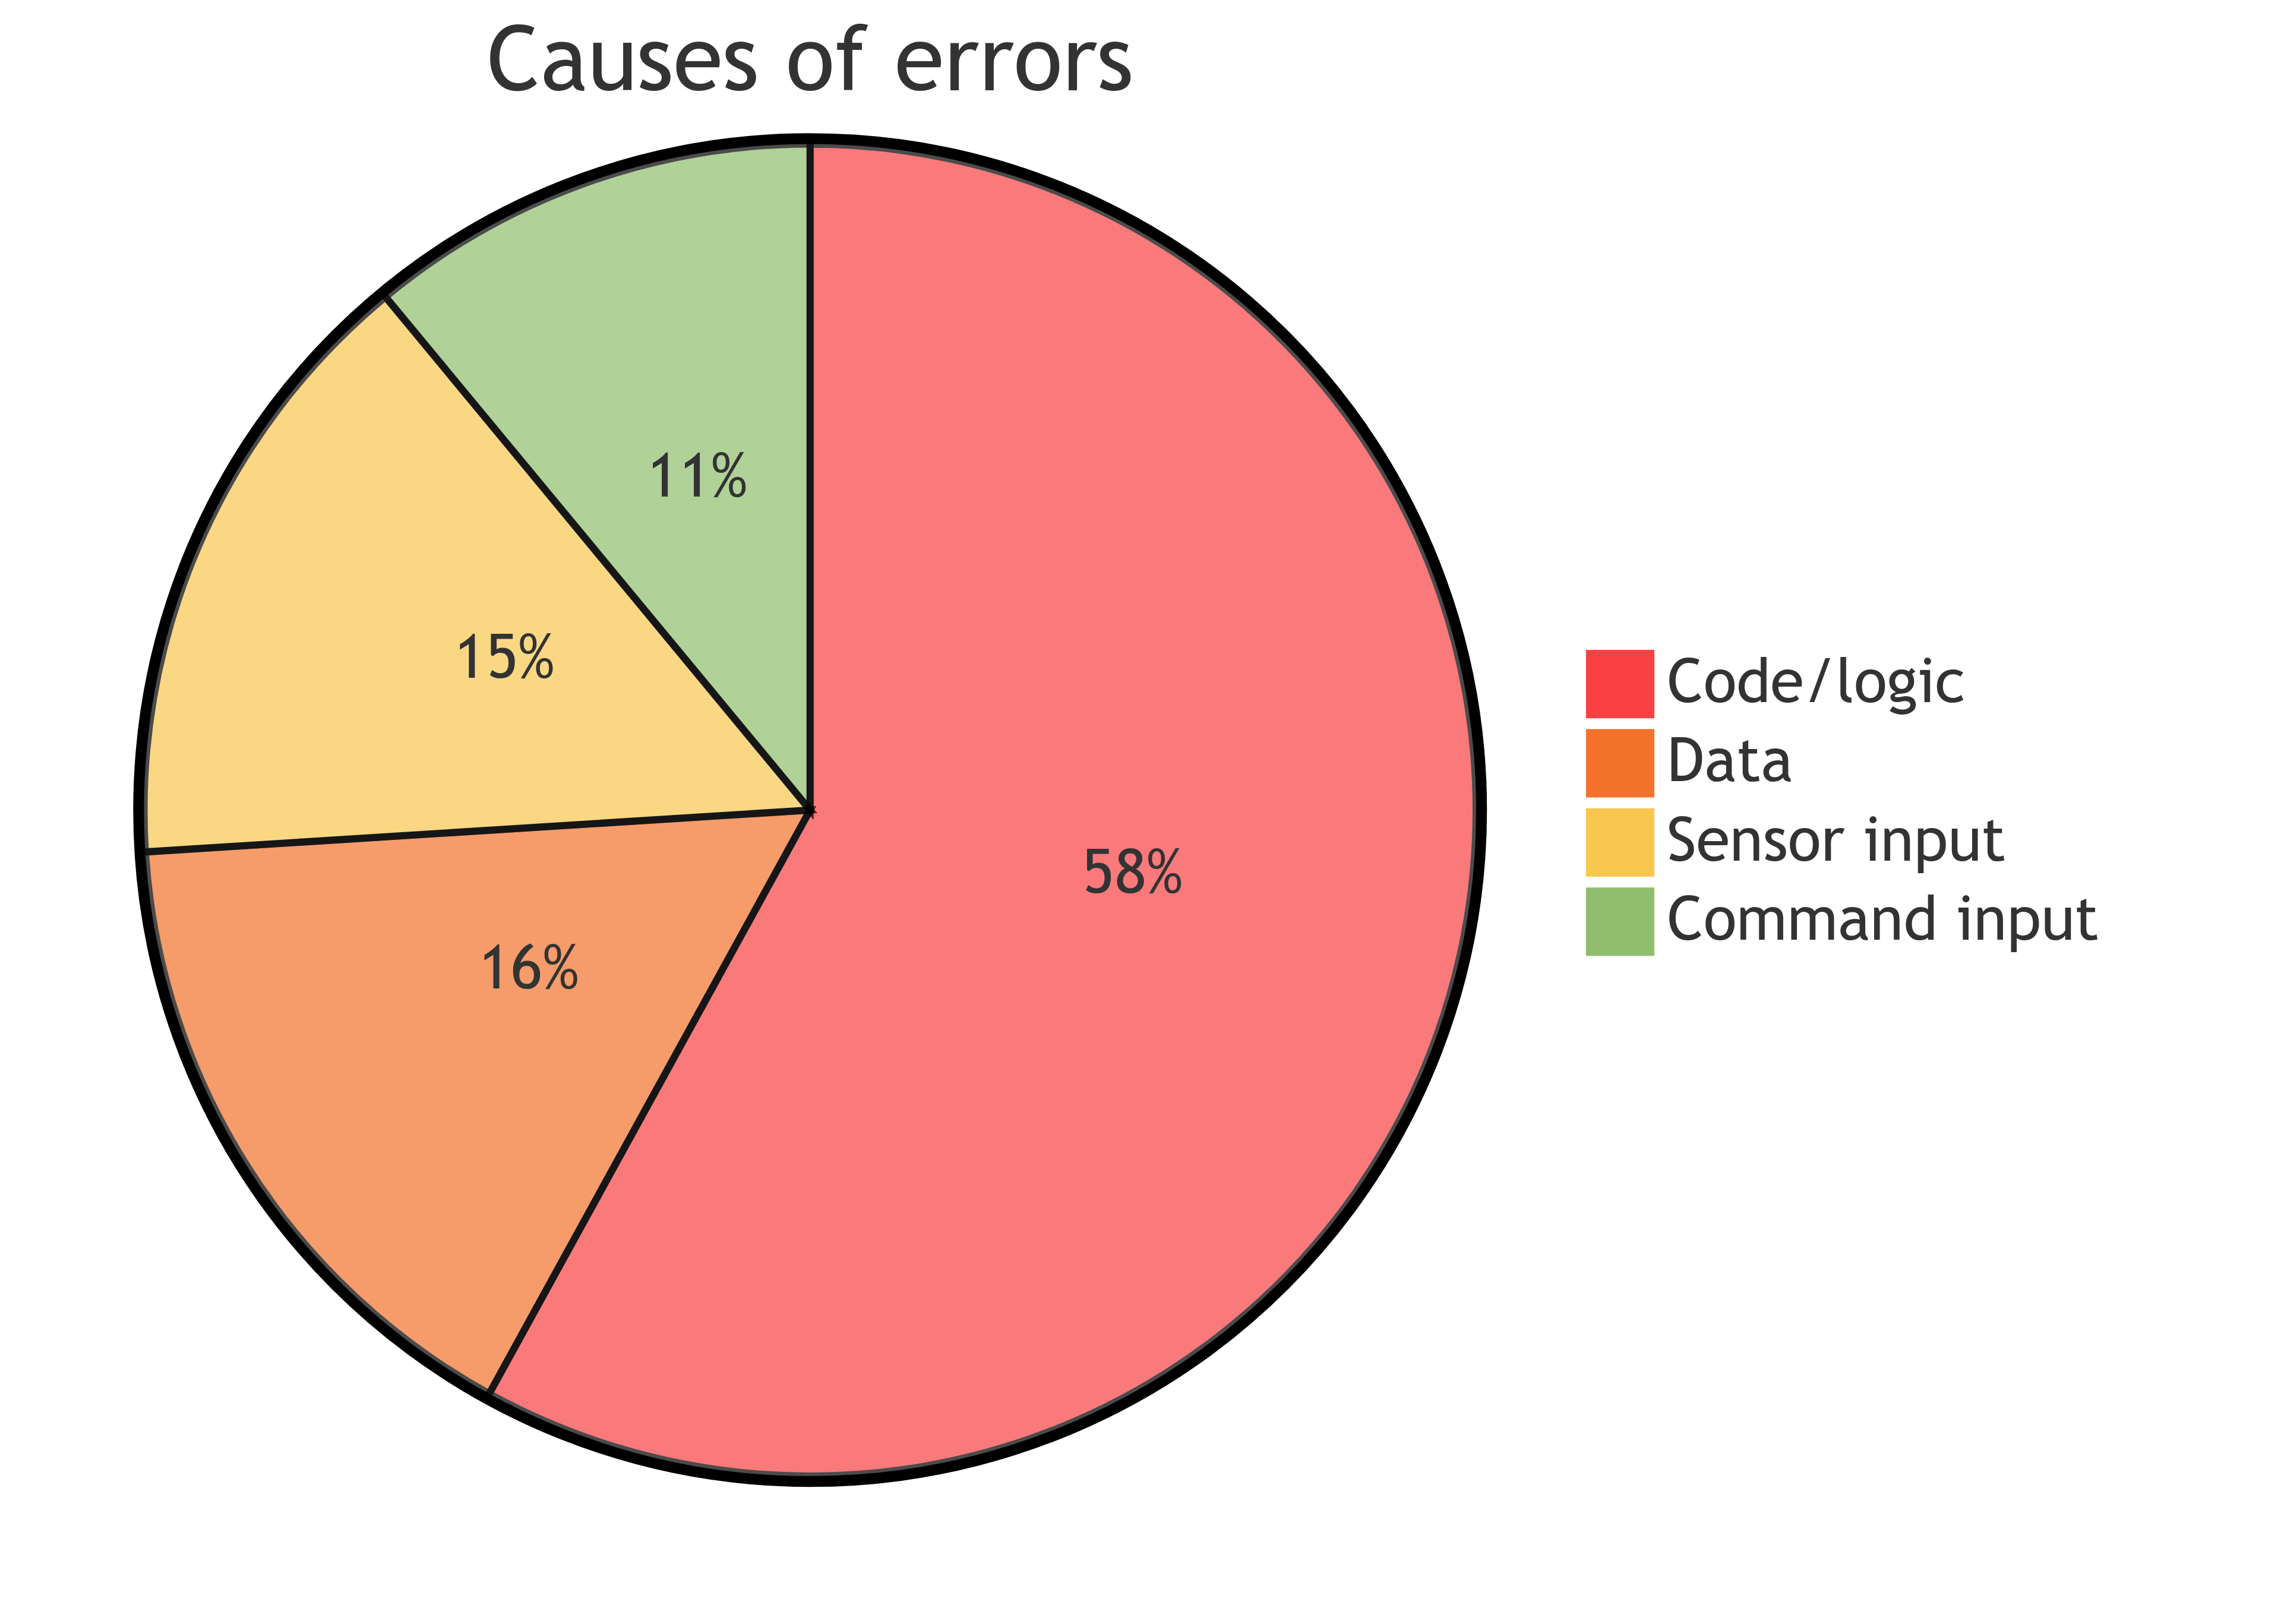
\includegraphics[width=0.7\textwidth]{diagrams/stats/piechart.png}
    \caption{Causes of errors}
    \cite{nasa:stats}
\end{figure}

To ensure that software remains robust and as free of errors as possible, there are several effective strategies. One promising approach we will look at is the use of memory-safe programming languages, specifically Rust. Rust is a modern language that has gained traction for its safety features, particularly in system programming and embedded applications. It ensures high performance through zero-cost abstractions and introduces a memory ownership model, which reduces memory-related errors such as null pointer dereferencing and data races. This model makes Rust particularly well-suited for low-level and resource-constrained environments, where reliable memory management is crucial. (https://docs.rust-embedded.org/book/) \\

\section{Fault tolerance techniques}

\subsection{Single version} \label{single}

Single version is a category of techniques which focus on creating a singular, robust implementation of software by integrating safety checks and redundancies directly into the software design process.

This technique emphasizes the detection of errors within the software and the ability to recover from them. Error detection typically involves monitoring the system for unexpected behaviors or inconsistencies, which could signal the presence of a fault. Recovery mechanisms then act to mitigate the effects of these faults.

Handling an error can be done in various ways. Most common would be to backtrack to a saved checkpoint and retry the part of the application where an error was discovered in the hopes of getting the correct result on the subsequent retries. This usually works well with transient faults, but it is likely to fail in the presence of a solid fault \cite{1402092}. 

Drawbacks of single version techniques are primarily the lack of alternatives and fallbacks, should the version fail. Single-version techniques heavily rely on error detection and recovery, which might not always work in practice. The reason single-version techniques are viable is an observation that transient errors are way more common than solid errors \cite{1676899}, meaning that single-version is sometimes enough for noncritical parts of the system.

\subsubsection{Modularity}

Perhaps the simplest way we can create a more resilient software is to structure it into independent modules. Each module should handle one task and, when possible, not directly rely upon any other modules for its functionality, or be relied upon by other modules.

A technique commonly utilized to achieve modularity is partitioning, which can be divided into horizontal and vertical partitioning. Horizontal partitioning aims to split the software into independent structural branches communicating through interfaces. 
Vertical partitioning splits the software in a top-down fashion, where higher level modules are tasked with control logic, while lower level modules do most of the processing \cite{nasa:sft}.

\begin{figure}[hbt!]
    \centering
    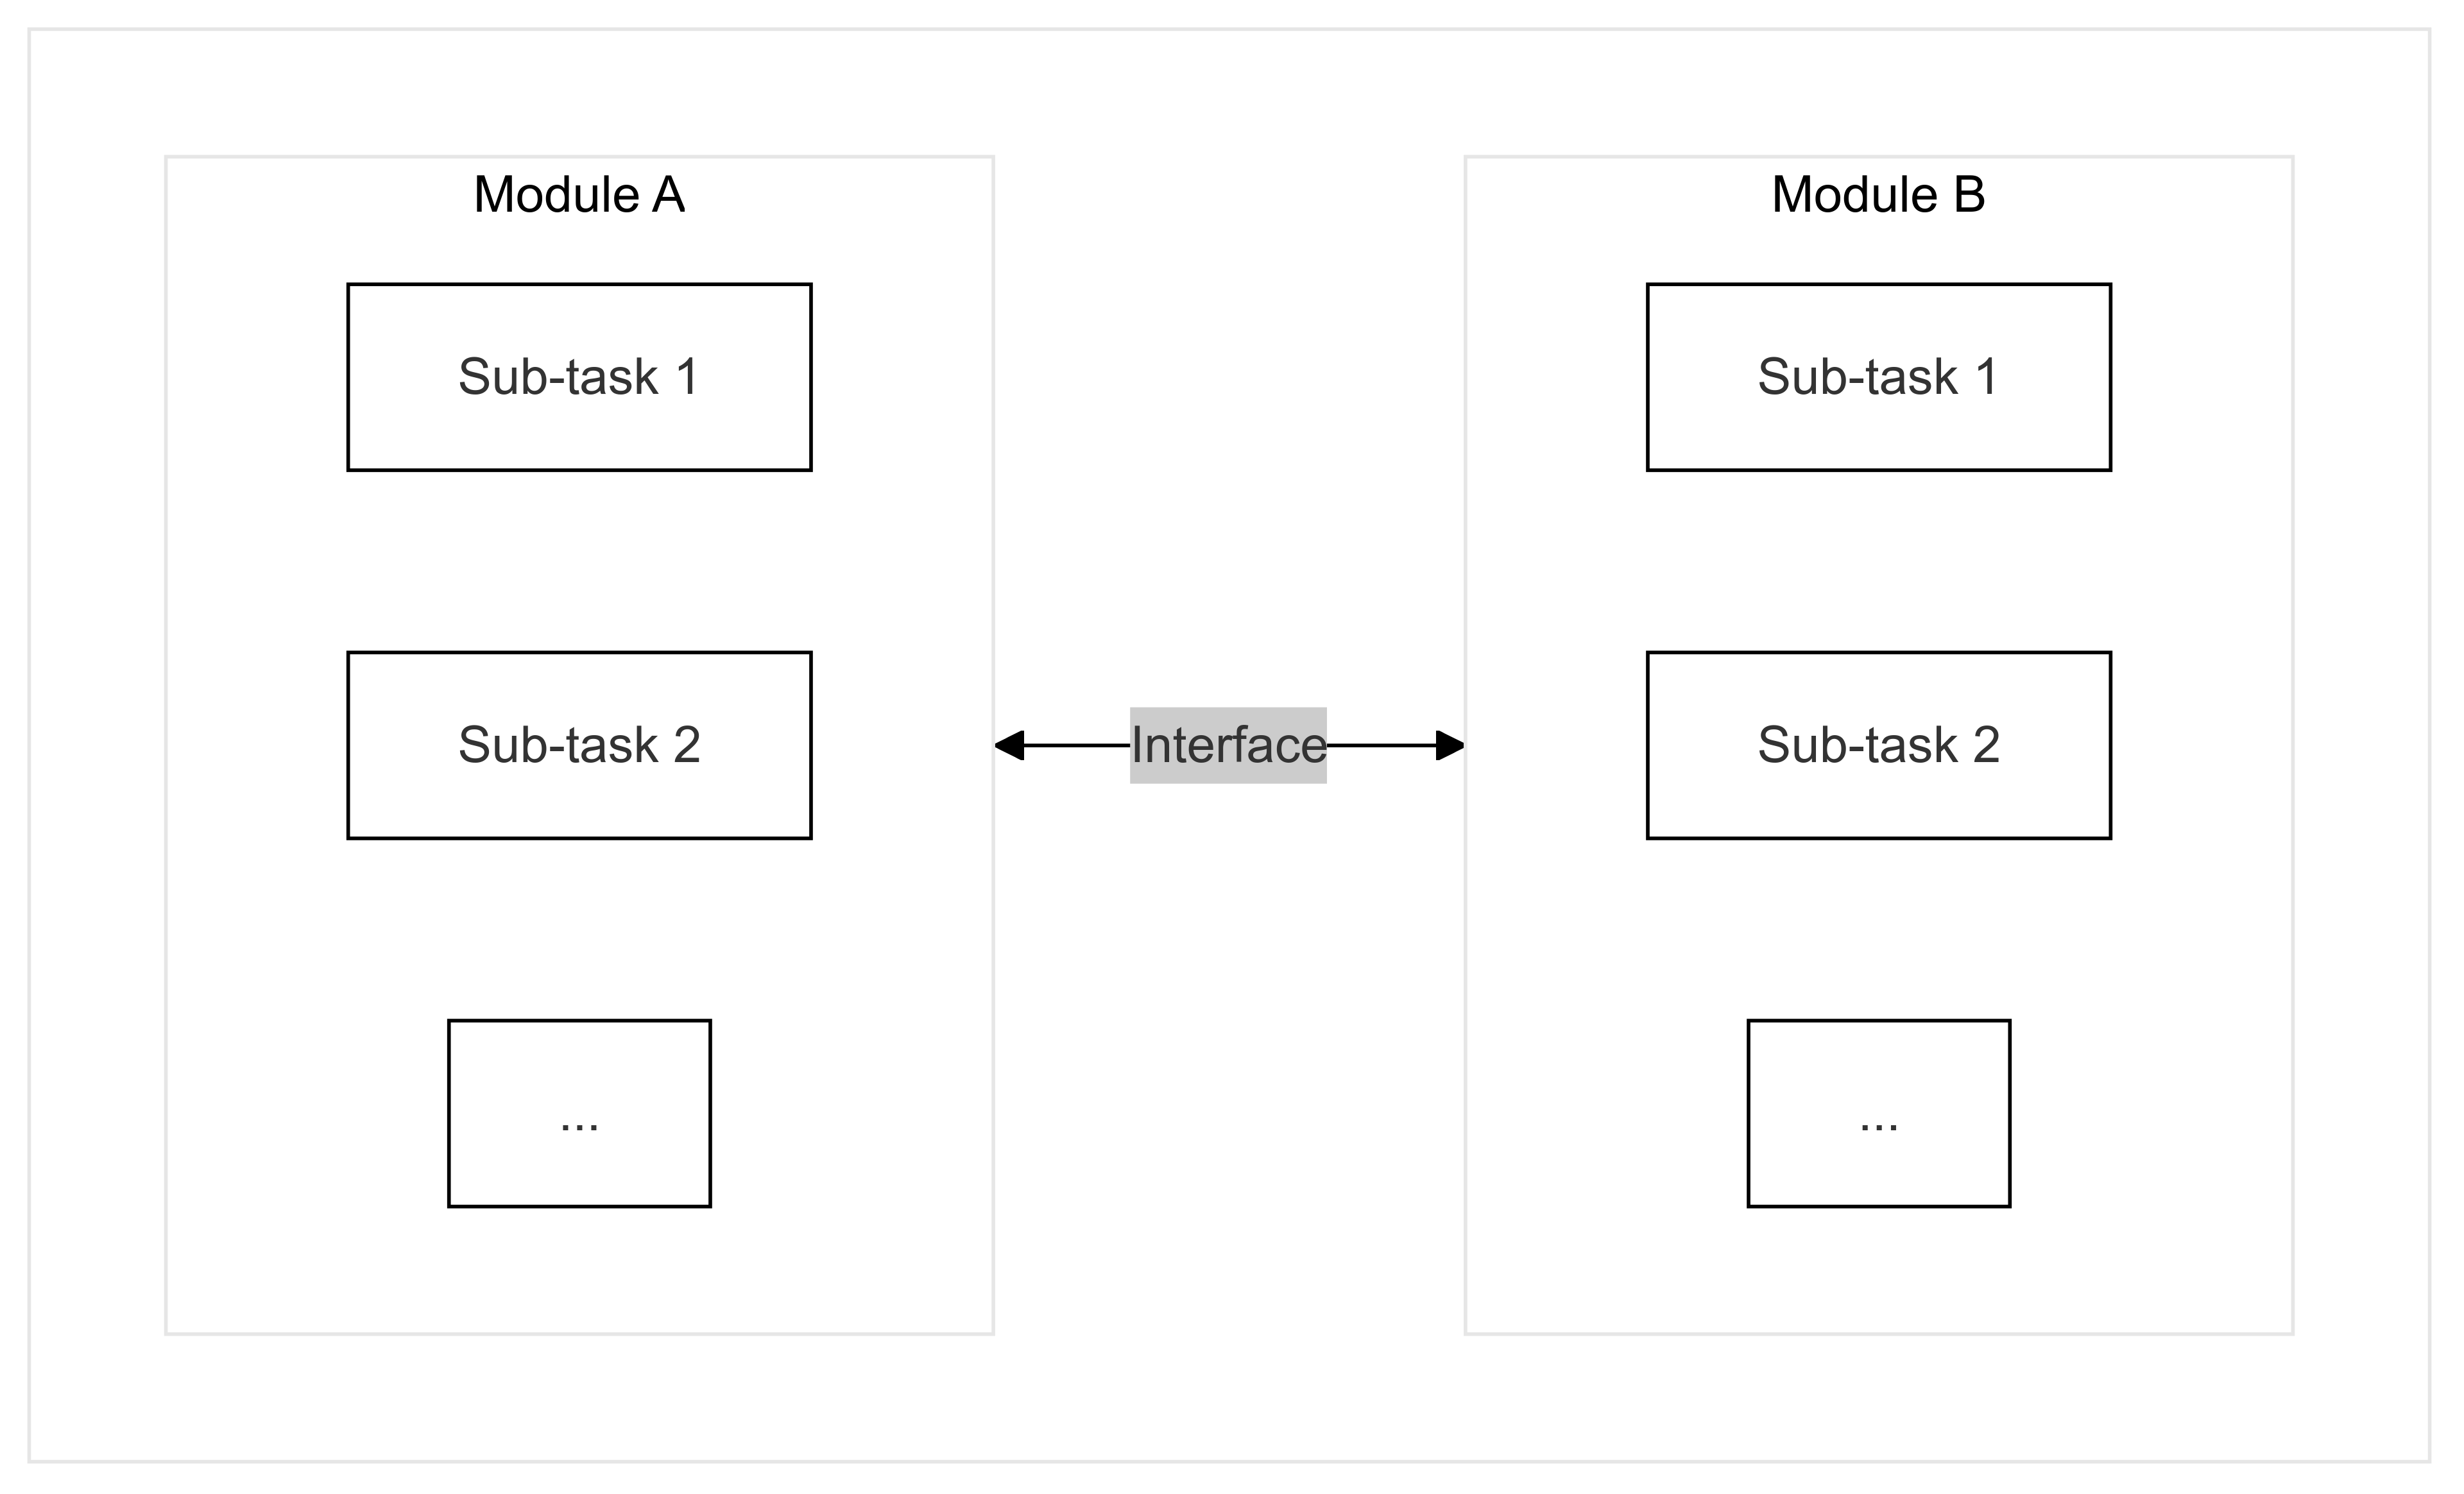
\includegraphics[width=0.7\textwidth]{modularity/horizontal.png}
    \caption{Horizontal partitioning}
    \label{fig:mod_hor}
\end{figure}

\begin{figure}[hbt!]
    \centering
    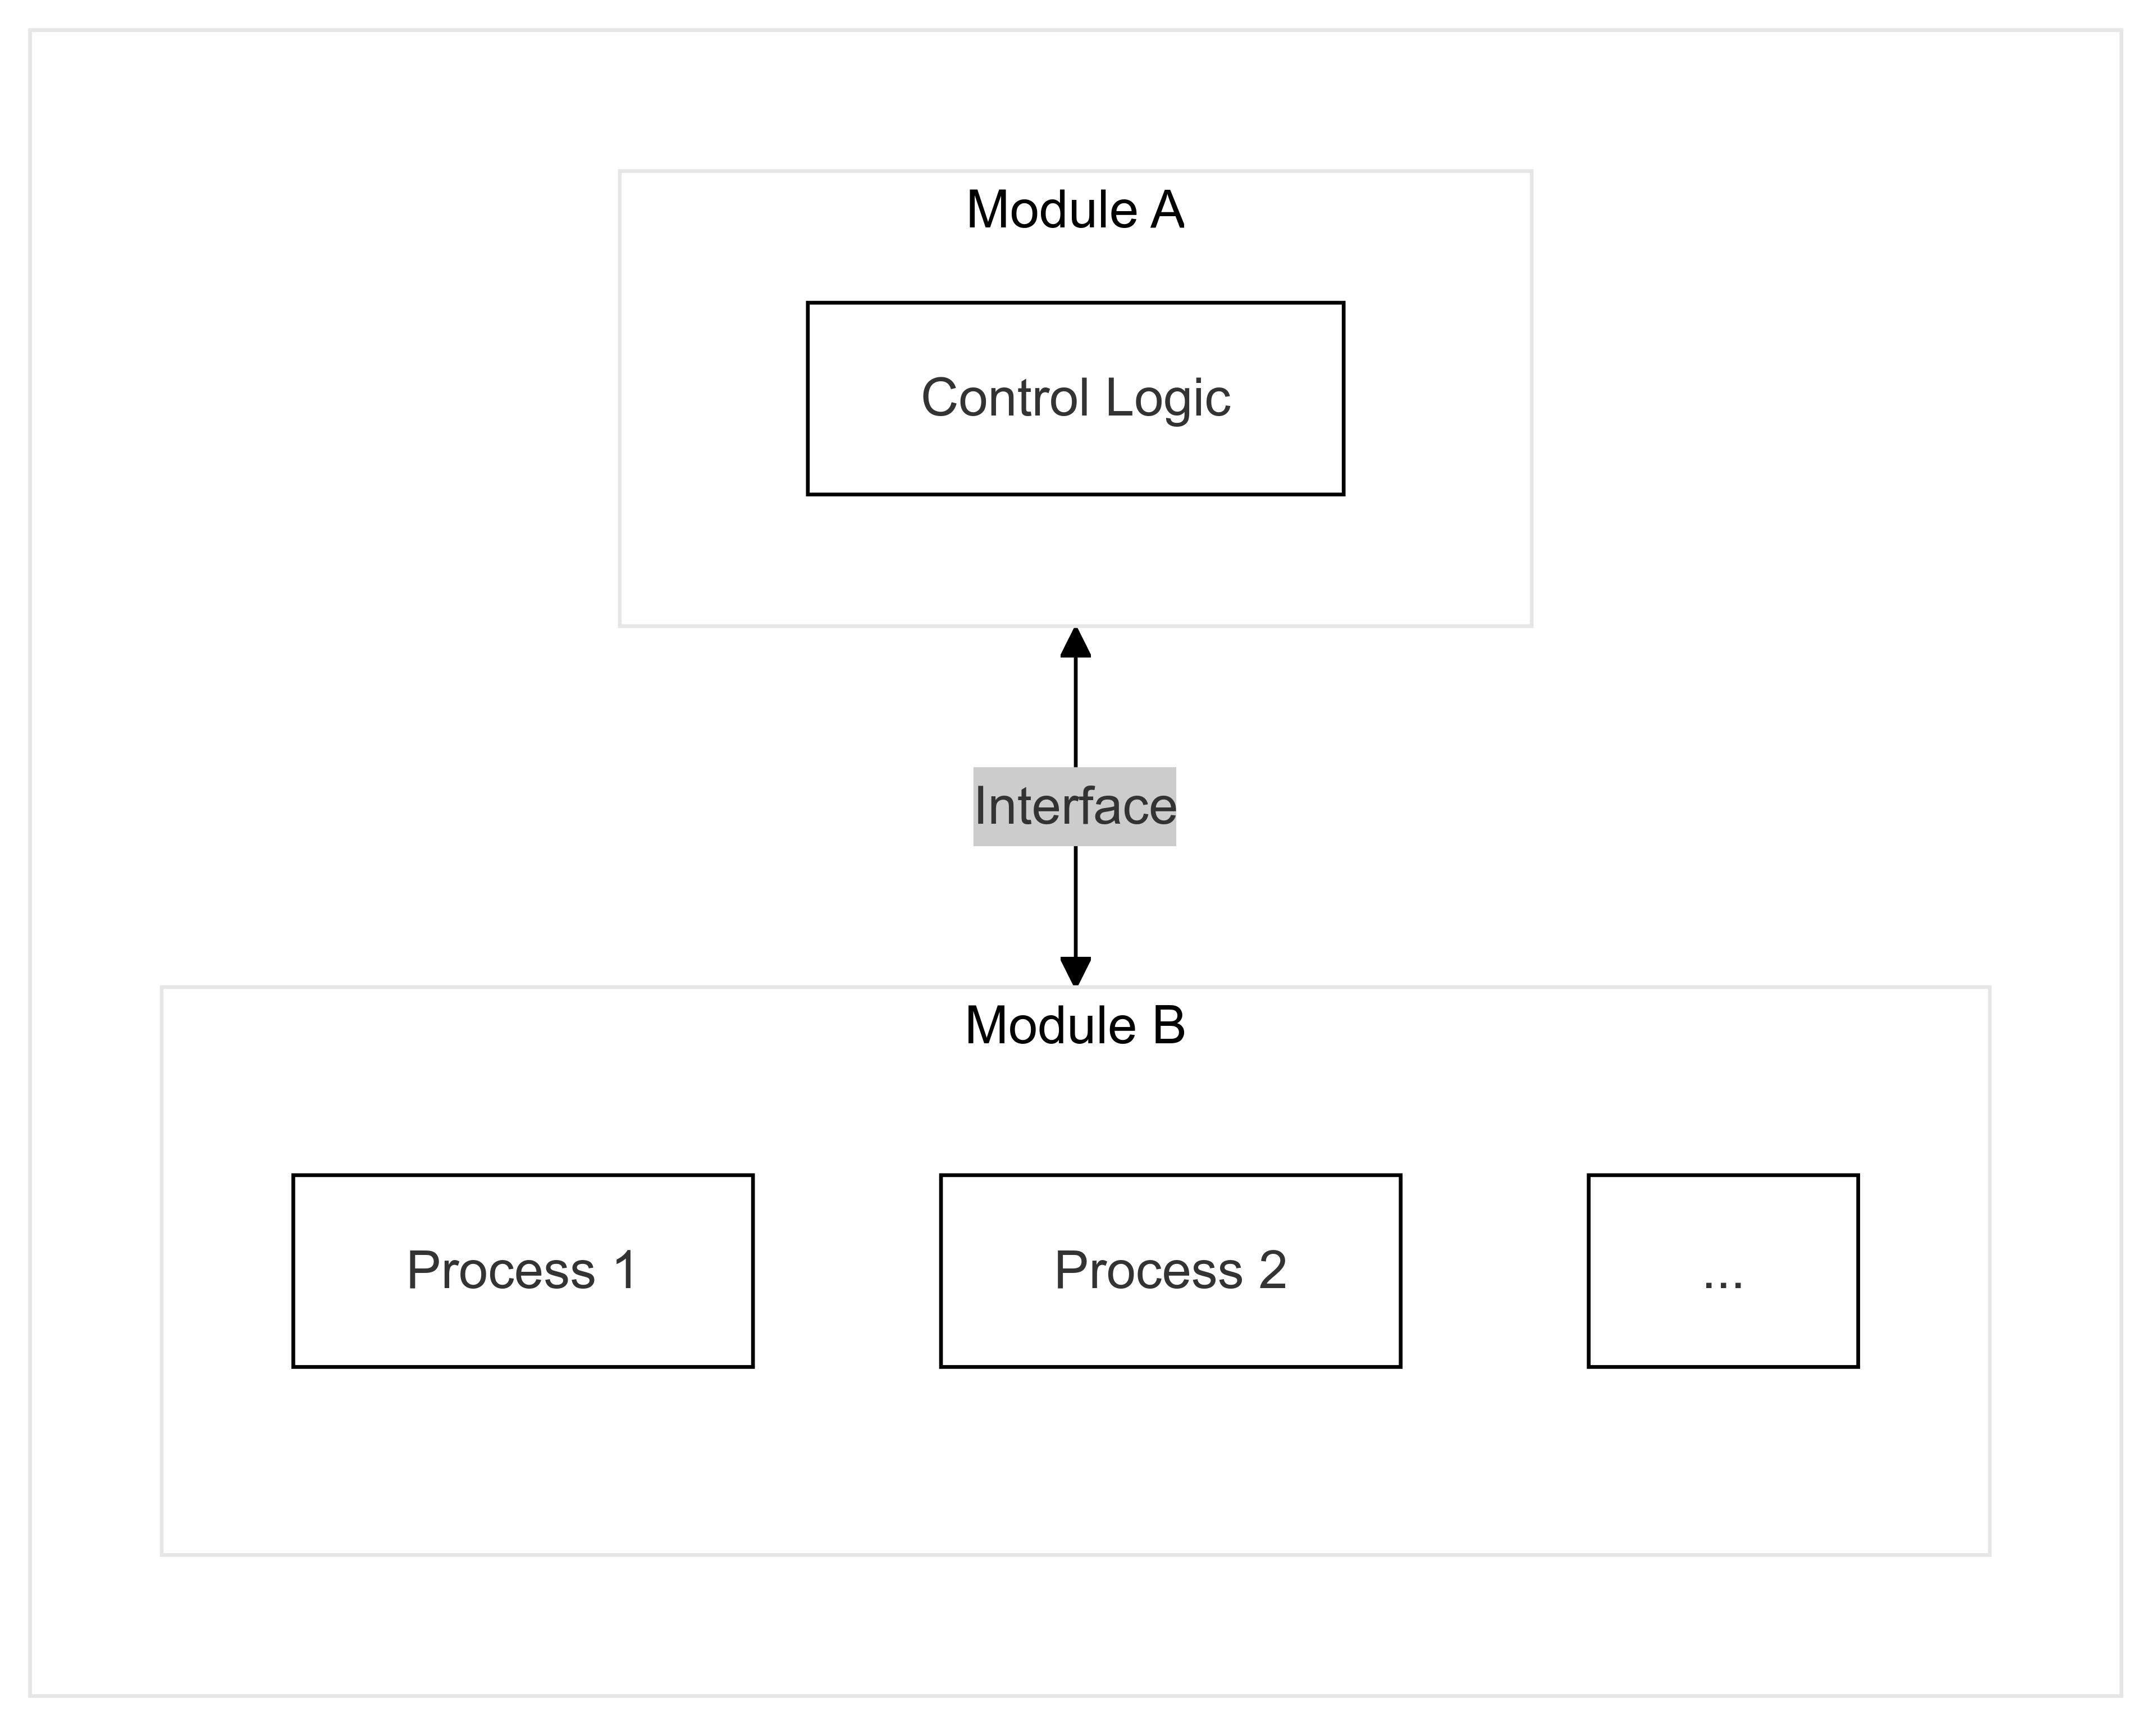
\includegraphics[width=0.7\textwidth]{modularity/vertical.png}
    \caption{Vertical partitioning}
    \label{fig:mod_ver}
\end{figure}

Benefit of partitioning is the ability of software to isolate errors. Provided the software is correctly structured, an error occurring in a single module should not propagate to other modules. Meaning we can use modularity as a way to pinpoint the erroneous parts of software and attempt recovery. If recovery is not possible, the software should still be able to partially function, given that other parts of the software are not influenced by the fault. In most situations, partial functioning of a software is preferable to a complete shutdown.

\subsubsection{Error detection}

Fault-tolerant single-version application should meet two main criteria: self-protection and self-checking. Self-protection means that the application should be able to protect itself from external corruption by detecting errors in information being passed into the application. Self-checking means that the application component must be able to detect errors within itself and prevent propagation of these errors into other components. These two traits combined can be together considered as the ability of "error detection".

Error detection covers a wide range of techniques used to locate errors and mitigate them. Some common approaches include:

a) checksums and error correction codes (ECC), which embed additional metadata with the actual data in order to verify integrity and attempt to correct corrupted data. This approach allows for some degree of memory corruption mitigation but comes at the cost of memory overhead and additional processing per data-chunk which uses checksum or ECCs.

b) assertion and runtime checks, which perform independent checks on the data during execution which ensures the data matches the expected outcomes at certain checkpoints. This approach also carries with it the additional processing overhead without guarantees that we will be able to catch all errors.

c) watchdog timers, whose main purpose is to catch deadlock states by giving a task a certain amount of time to execute before aborting it.

Error detection is a crucial aspect of single-version application, since we have no alternate version to fall back upon.

\subsubsection{Checkpoint and restart}

Checkpoint and restart could be considered the basis of some of the more advanced fault tolerance techniques. It involves creating a data checkpoint which the software can be rolled back to before the execution of a process. At the end of the execution, an acceptance check is performed on the process output, if an error is detected rollback is initiated and the process is restarted.

\begin{figure}[hbt]
    \centering
    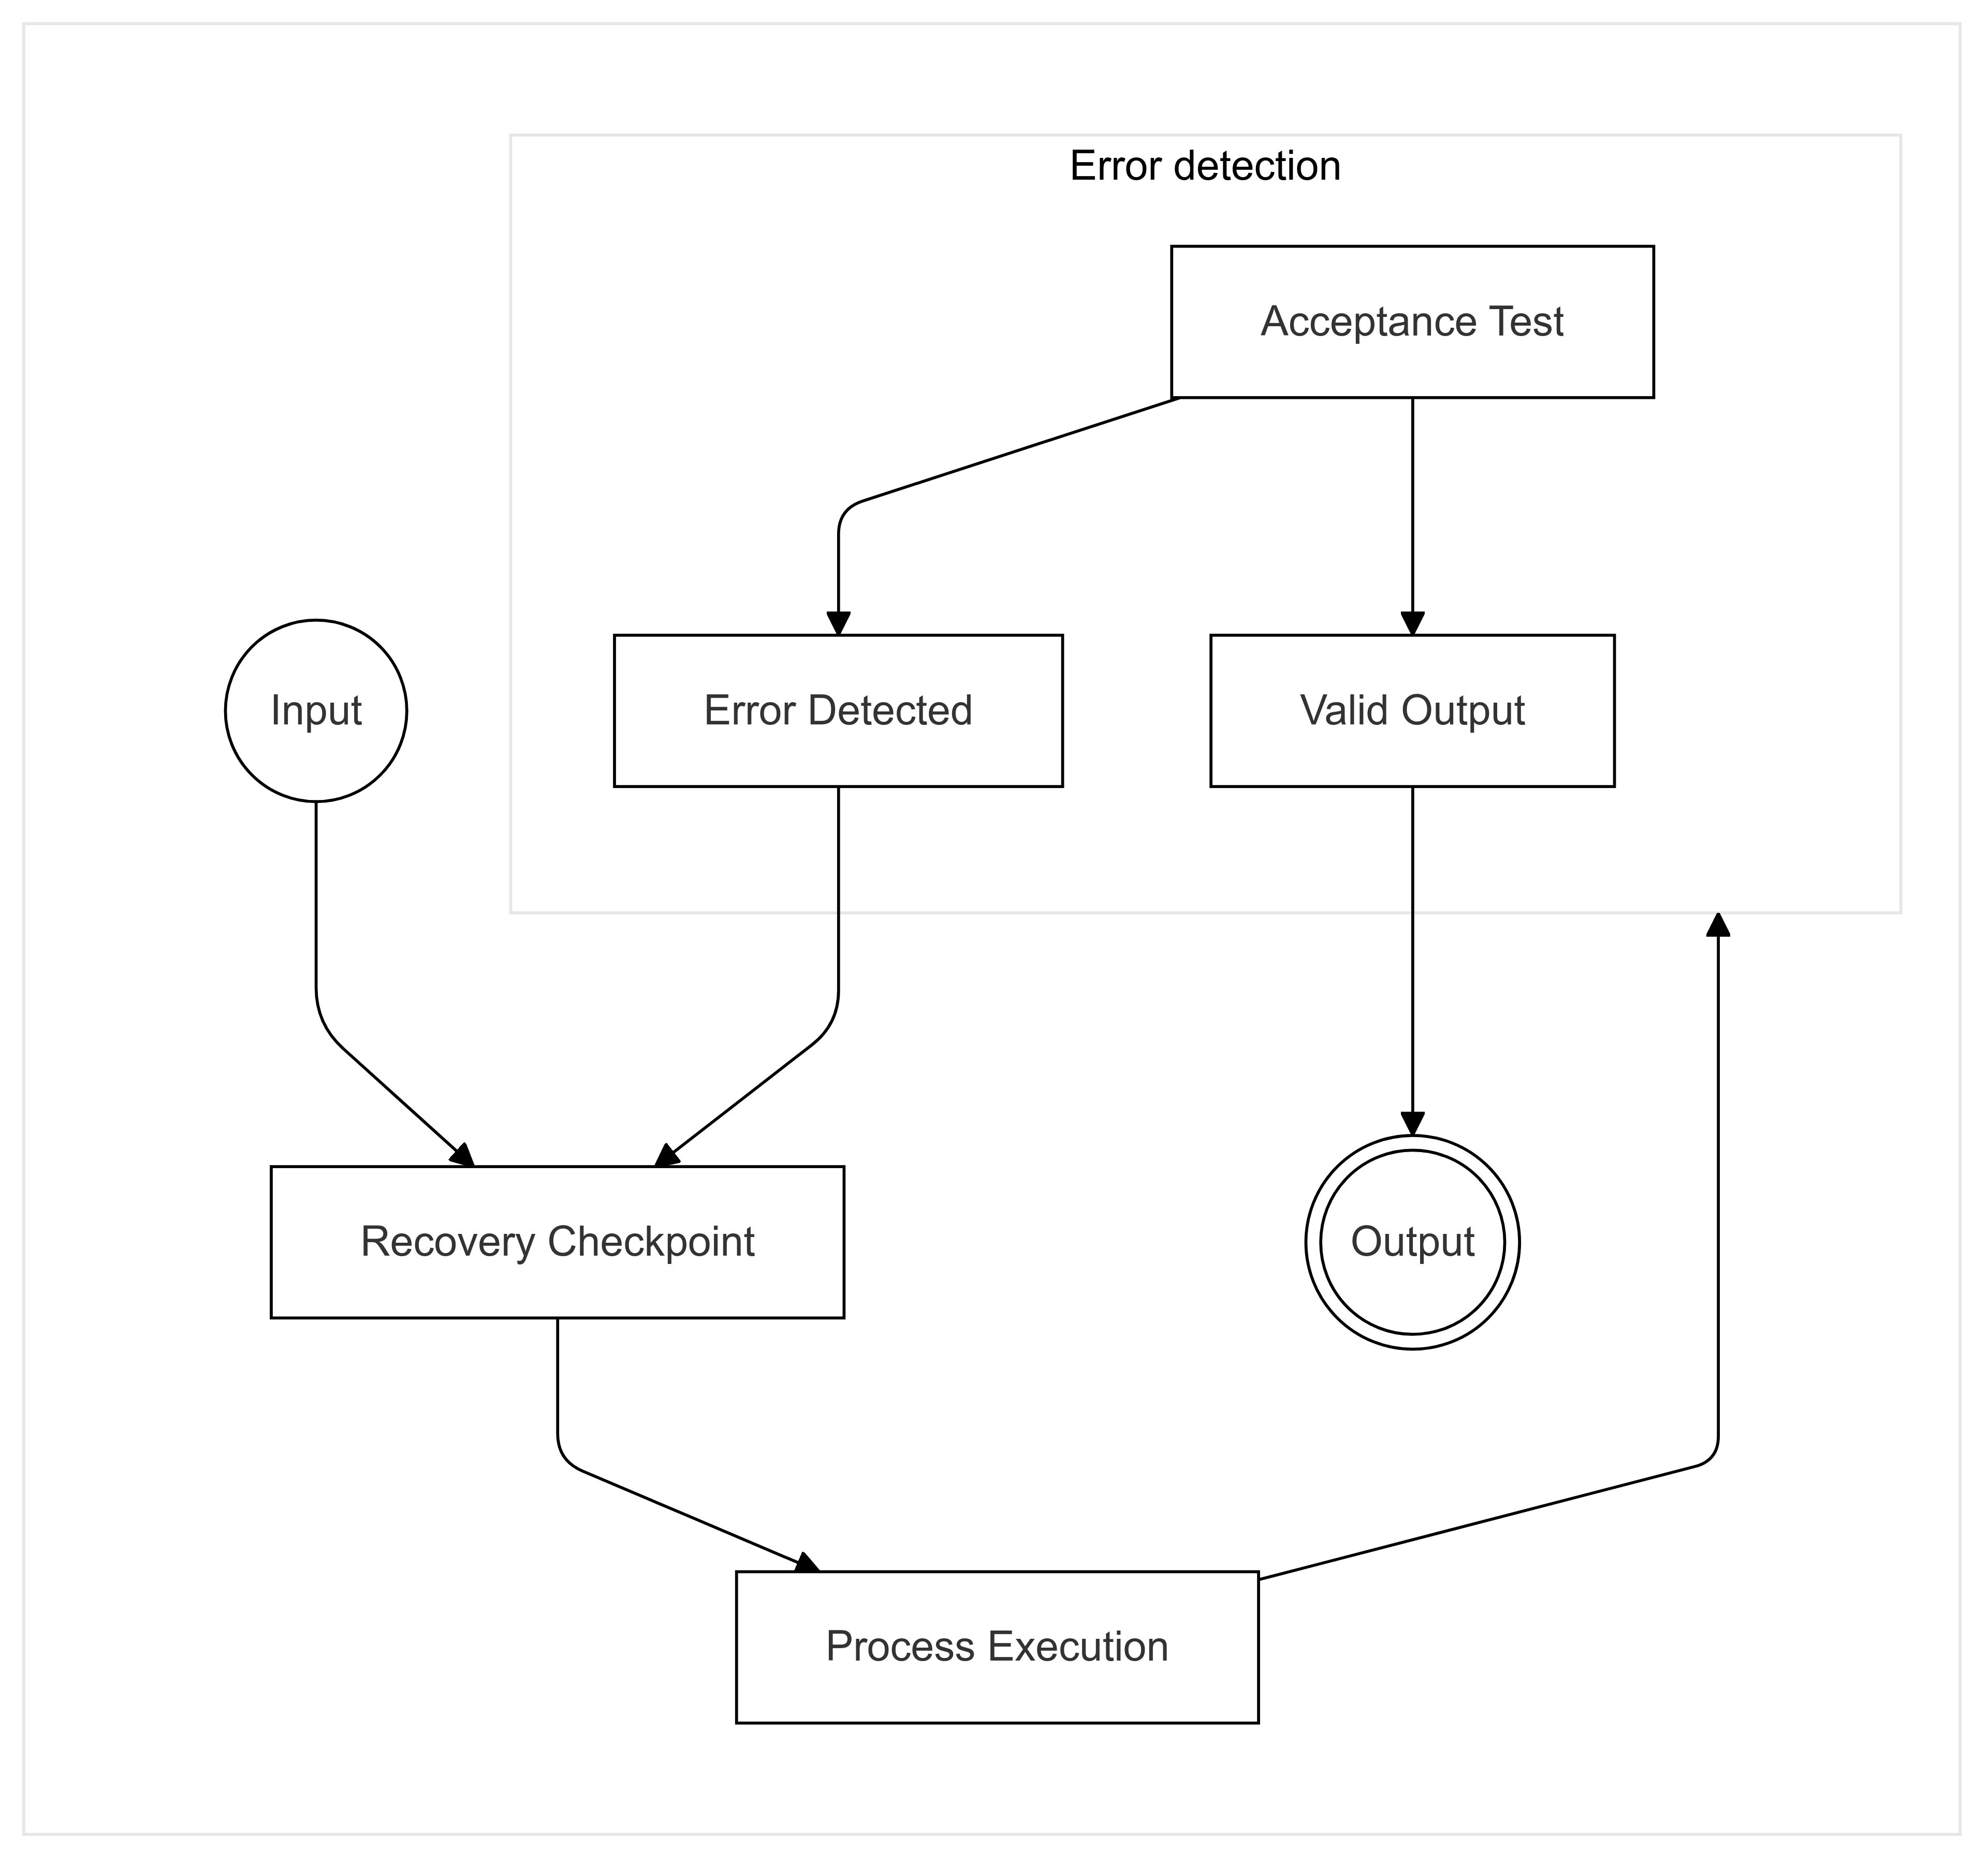
\includegraphics[width=0.8\textwidth]{diagrams/checkpoint/checkpoint.png}
    \caption{Checkpoint and restart}
    \label{fig:checkpoint}
\end{figure}

\subsubsection{Considerations for single version techniques}

Single version fault tolerance techniques are largely easier to develop when compared to the ones discussed in the following section. With this relative simplicity comes the drawback of being ill-suited for some situations. While these techniques should work well for transient faults that are unlikely to reoccur, a single version fault tolerant system will fail when attempting to deal with persistent faults. Even if an error is successfully detected, single version techniques provide no clear way of dealing with errors that stem from, or are heavily influenced by the design of the system. As an example, if the memory region containing a critical function has been permanently damaged, it matters not how many times we attempt to rerun said function, it will always cause an error. For this reason, single version techniques should be reserved for parts of software which are not mission critical and allow system to function even in their absence.

In order to effectively deal with solid faults, we need to consider multi-version techniques covered in the following section. A lot of these techniques take inspiration from single version techniques, or even directly build off of them.

\subsection{Multi-version} \label{multi}

Multi-version techniques build on the idea of multiple software versions which all meet the same specifications. These versions are interchangeable in terms of their output, but each version executes differently from the rest, ensuring that no two version share the same failure regions.
Multiple versions of the same software are executed either in sequence or in parallel, each utilizing different error detection and recovery methods, to have the highest probability of at least one completing the task successfully.

\subsubsection{Recovery blocks}

Recovery blocks is a simple form of multi-version programming, expanding upon the idea of "checkpoint and restart". Unlike its single version counterpart, however, recovery blocks does not re-execute the same code again, but instead chooses a different version to try next.

A key advantage of the recovery blocks technique is that, in most cases, the initial version will execute successfully, allowing subsequent versions to prioritize redundancy and safety over performance. This enables the design of backup versions with gradually reduced performance requirements, ensuring robust fallback options without excessive resource consumption.

\begin{figure}[hbt!]
    \centering
    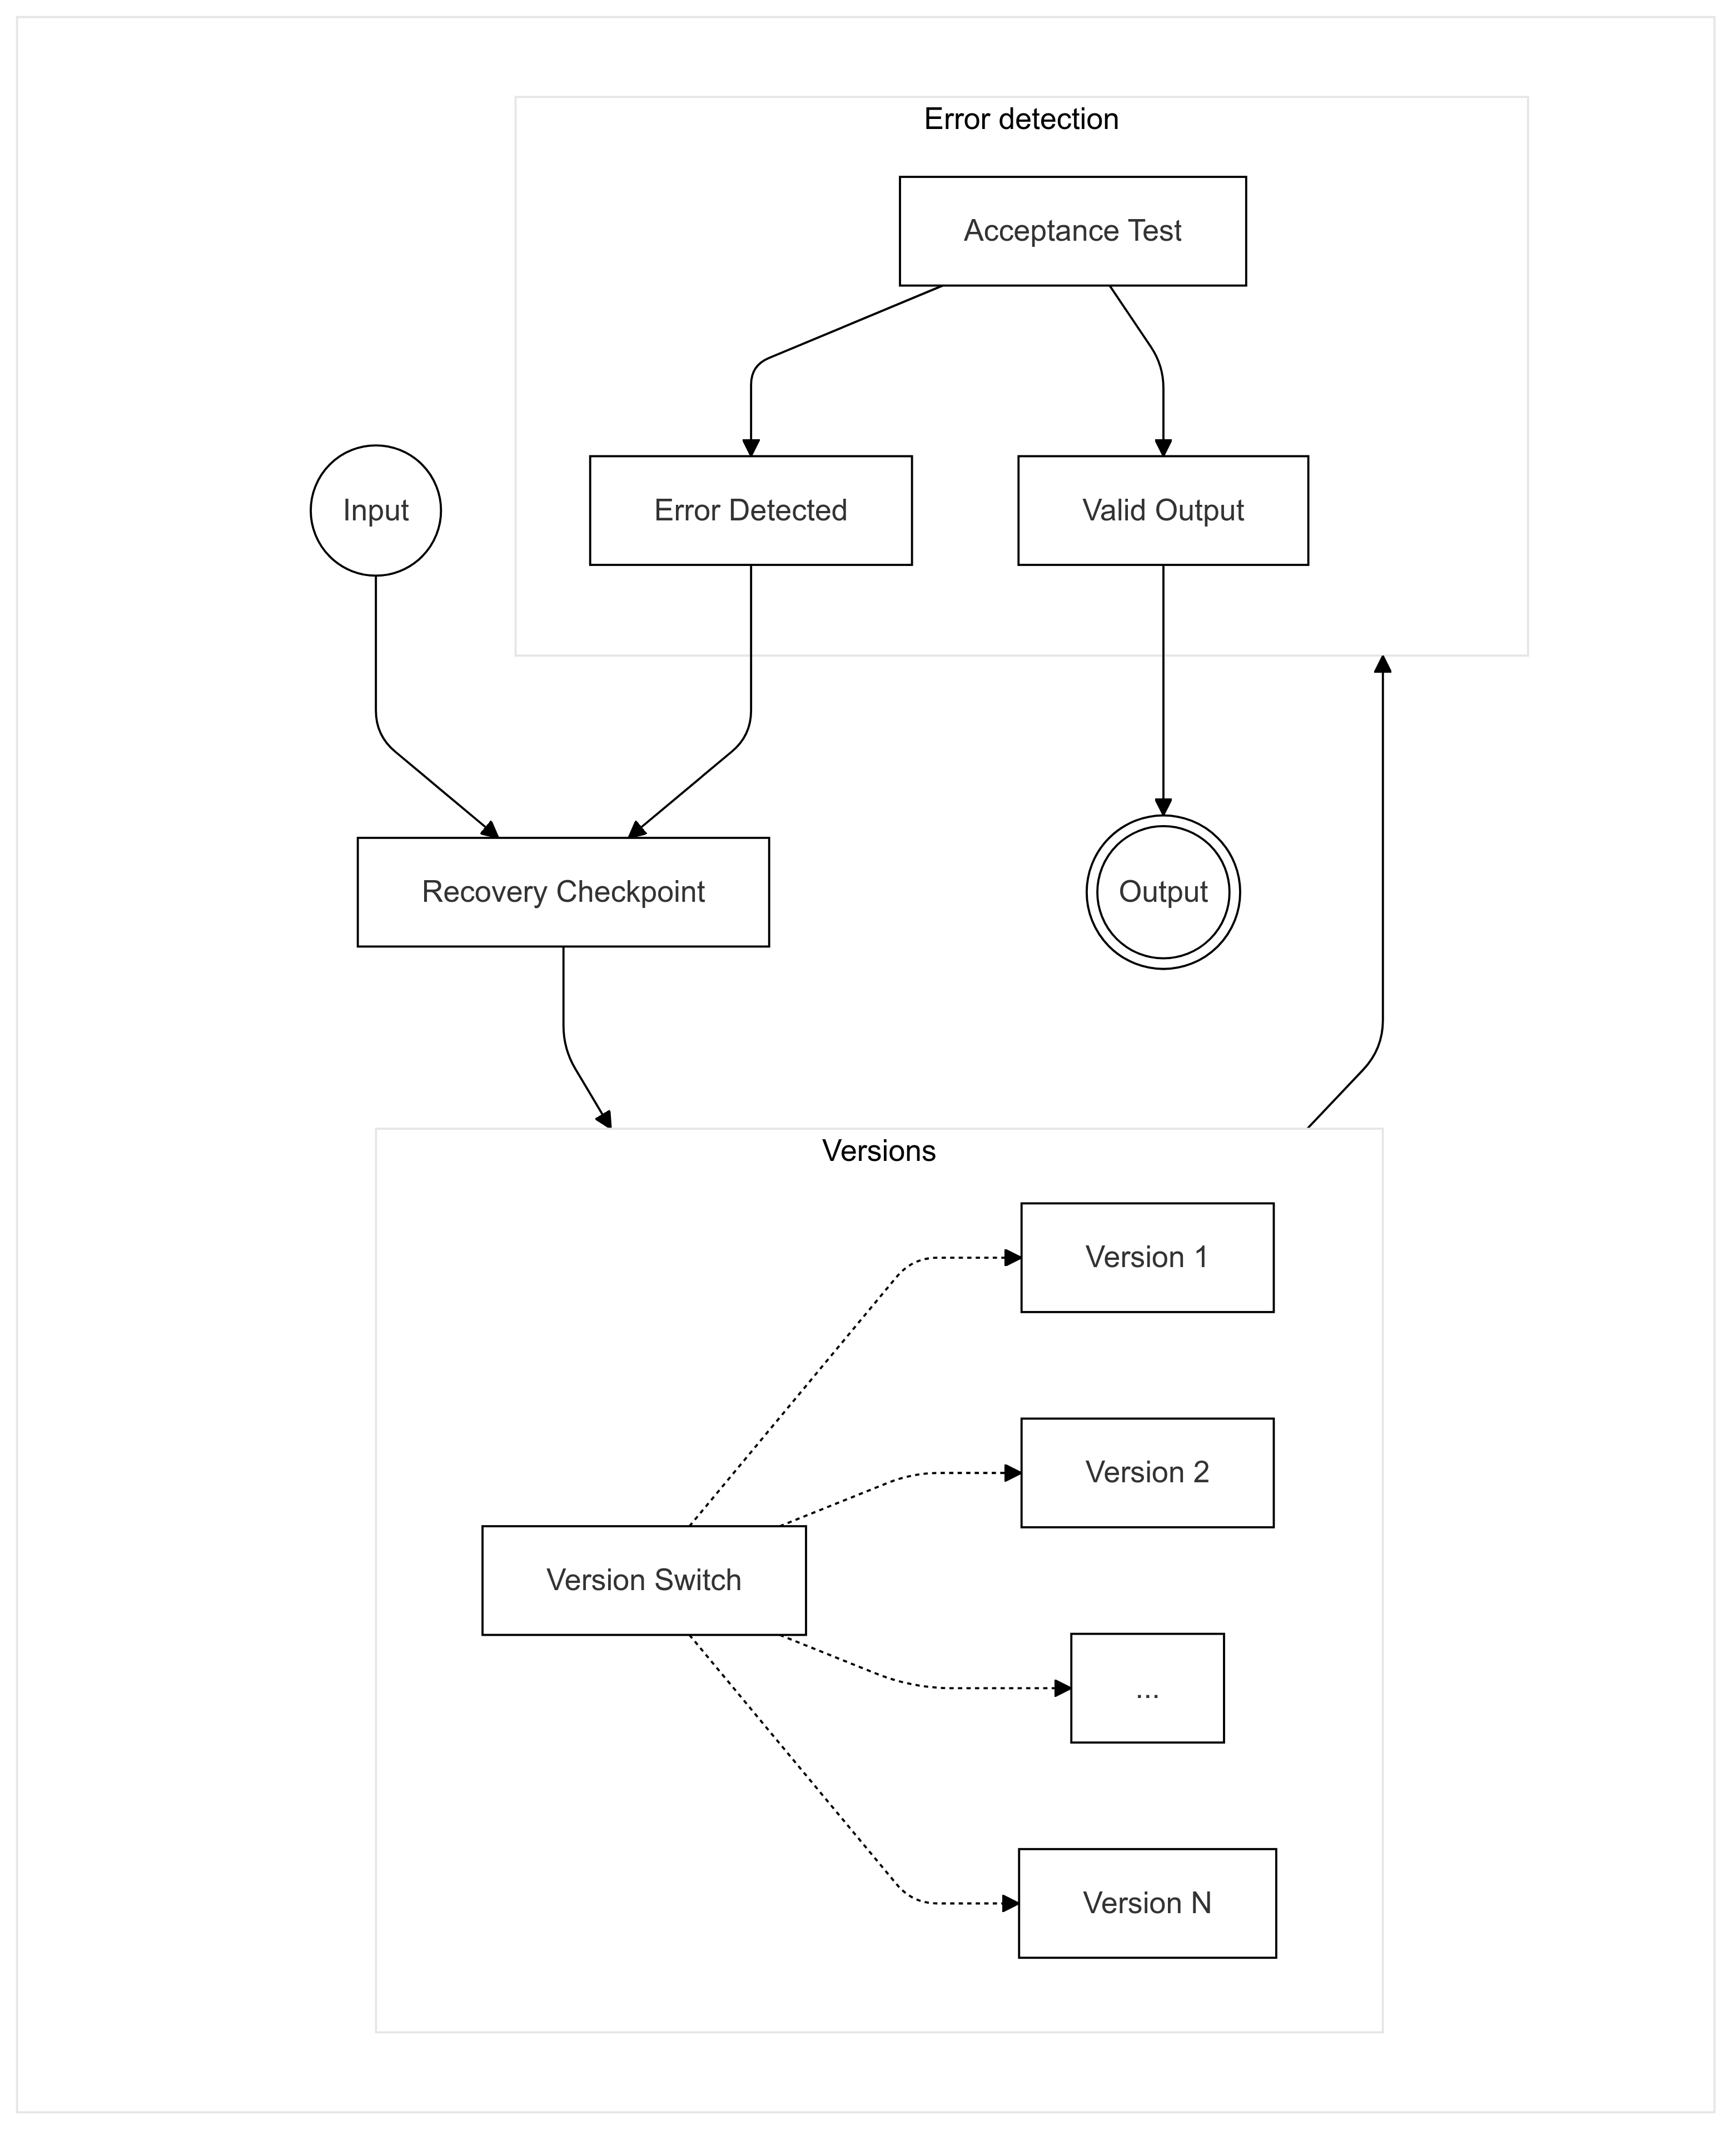
\includegraphics[width=0.9\textwidth]{recovery_blocks/recovery_blocks_01.png}
    \caption{Recovery Blocks}
    \label{fig:rec_blo}
\end{figure}

\break

\begin{lstlisting}[language=Rust]
// Exectutes version based on the version ID
async fn version<T, U>(ver_id: u32, input: T) -> U {
    ...
}

// Validates the version output based on the input
fn acceptance_test<T, U>(input: T, output: U) -> Result<U> {
    ...
}

// Selects a different version based on the error 
// received from the acceptance test
fn version_switch<E>(error: E) -> u32 {
    ...
}

fn main() {
    /* 
    In a lot of cases, the input will be more complex 
    than just a single number, so before executing the version
    we would create a "data checkpoint" that would be restored
    before trying a different version.
    */
    let input = 42;
    let mut ver_id = 1;

    let correct_result = loop {
        match acceptance_test(input, version(ver_id, input)) {
            Ok(output) => break output,
            Err(error) => ver_id = version_switch(error),
        }

        if ver_id > MAX_VER {
            panic!("No version executed successfully");
        }
    }
}
\end{lstlisting}

Since errors are relatively rare compared to normal execution, this approach often achieves an optimal balance of performance and reliability. By prioritizing efficiency in the primary execution path while incorporating progressively resilient alternatives, recovery blocks can provide dependable fault tolerance without compromising system performance in typical operating conditions. This balance makes recovery blocks a practical solution for systems requiring high availability and reliability.

A consideration for recovery blocks is the utilization of a single shared acceptance check for all the versions. This means that the acceptance check must be implementation agnostic and only consider the inputs and outputs of the version. Although this means easier development and potentially less opportunities for faults given less software design, it also fails to take advantage of version-specialized ways errors could be detected in theory.

A considerable drawback of recovery blocks approach is its inherent complexity which creates numerous failure points. Namely, during error detection and state recovery. Since we are performing error detection on a singular execution of a version, we have no way to detect errors which coincide with normal functioning of the software, e.g. random bit flips in used variable. Errors such as these would result in incorrect output from a version, but would be undetectable provided the memory corruption is minimal. Even if we do detect an error, we have no guarantee that the state which was saved is not corrupted as well. We would need to employ various techniques to detect a corrupted recovery checkpoint and ideally implement redundancies to ensure the state can be restored.

\subsubsection{N-version programming}

N-version programming extends the multi-version technique by running "N" independent versions in parallel or in sequence, hence “N-version” programming. In this approach, each version meeting the same specifications independently performs the task, and the final outcome is determined through a consensus mechanism that evaluates the results from all N executions.

This consensus is usually achieved through a voting algorithm, which aggregates the outputs from each version and selects the result agreed upon by the majority. Selection algorithms are an entire topic of its own covered well by \cite{Aljarbouh_2021}.

This voting approach to handling errors is sometimes referred to as \textbf{fault masking}, since we are not necessarily concerned with detecting an error, but rather getting an acceptable output even in the presence of a fault.

\begin{figure}[hbt!]
    \centering
    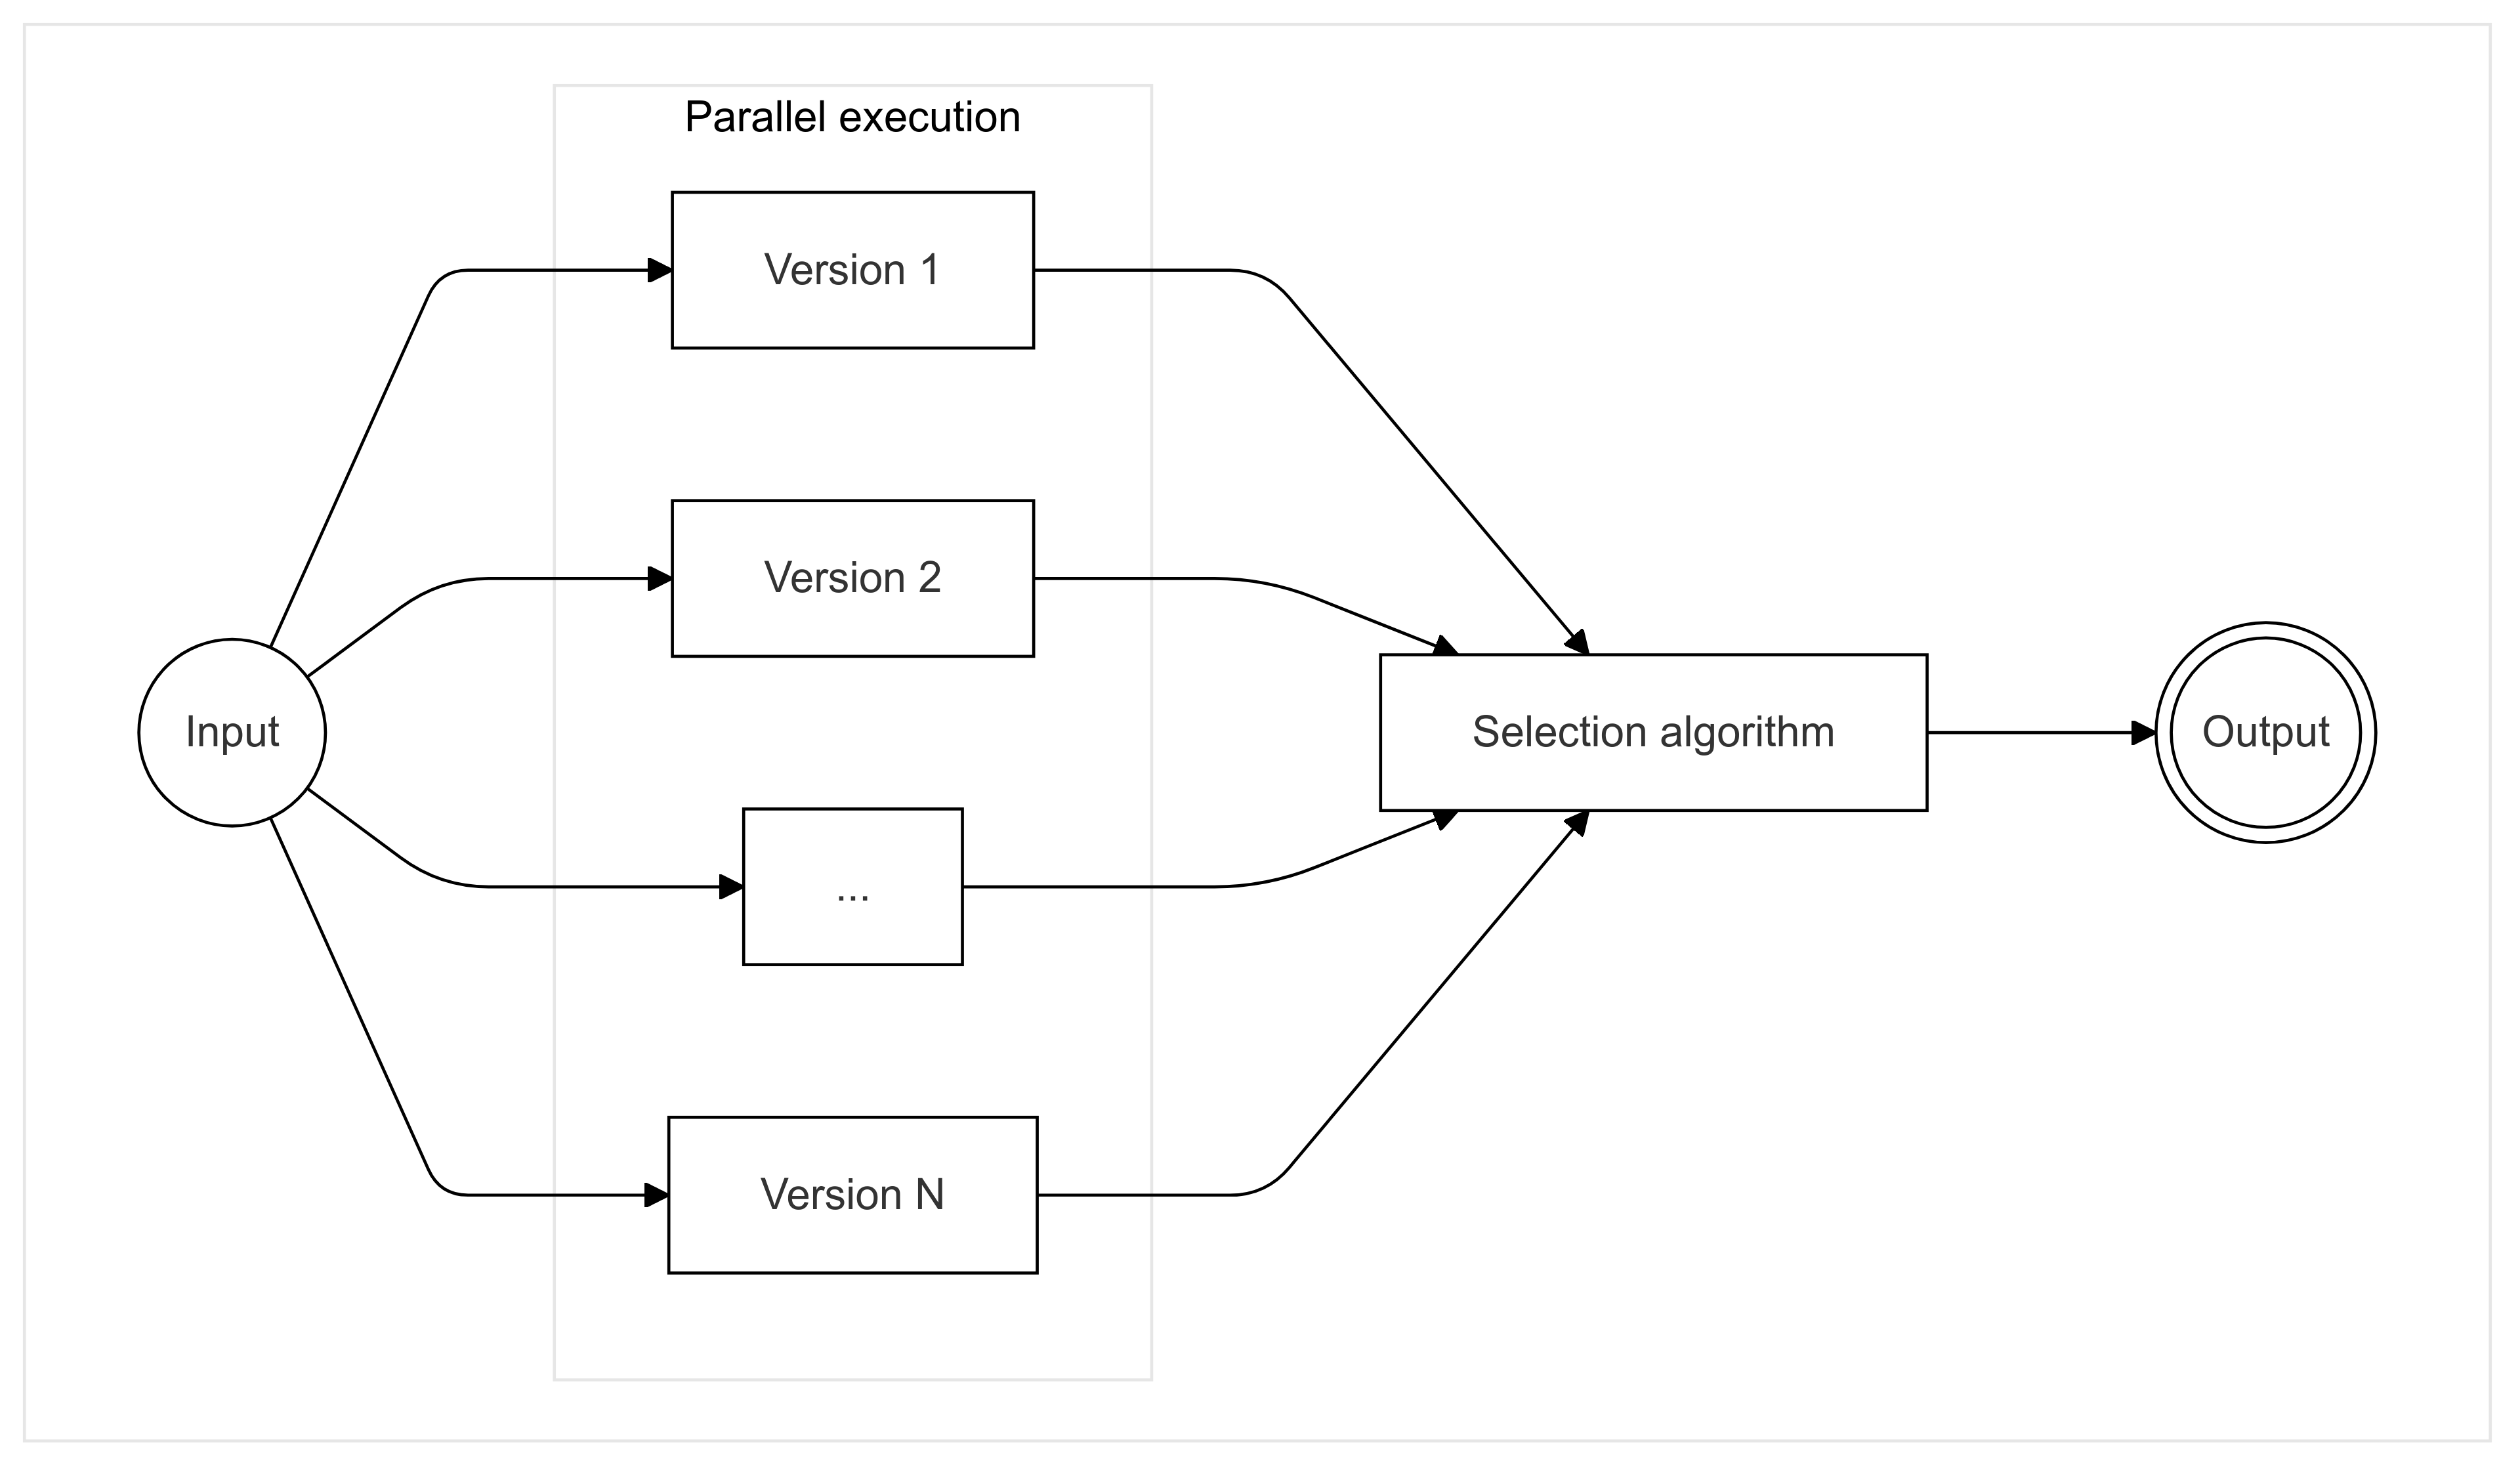
\includegraphics[width=0.9\textwidth]{n_version_prog/n_version_prog.png}
    \caption{N-Version Programming}
\end{figure}

\begin{lstlisting}[language=Rust]
async fn version<T, U>(ver_id: u32, input: T) -> U {
    ...
}

fn selection<U>(results: Vec<U>) -> U {
    ...
}

fn main() {
    let input = 42; 
    
    let results = futures::join!(
        version(1, input), 
        version(2, input), 
        version(3, input)
    );

    let correct_result = selection(results);
}
\end{lstlisting}

The primary drawback of N-version programming is its requirement to execute all of the versions before determining the final output. This can be highly resource-intensive, especially for large or complex tasks, as it requires significant computational power and memory to run multiple versions simultaneously.

For systems with limited resources, such as embedded systems, this approach can be particularly inefficient. The need to allocate resources for each version can strain the system's capabilities, potentially reducing its overall performance and responsiveness. As a result, while N-version programming enhances fault tolerance and reliability, it may not be suitable for applications where resource constraints are a priority or where processing efficiency is critical.

A consideration for N-version programming is the possibility of an error not being a random event, but rather a function of the input variables \cite{5326}. Therefore, even multiple versions running in parallel could all fail and give erroneous results. This makes the selection algorithm a critical failure point which N-version programming on its own does not address.

\subsubsection{N Self-checking programming}

N Self-checking programming is an extension of the classic N-version programming, where on top of executing multiple versions, each version also contains its own independent acceptance test or recovery block, before the results are passed to the selection logic. The selection logic then selects the "topmost" possible version that reports a correct output.

A version-specialized acceptance check is an interesting addition, as it provides the opportunity to take advantage of the version implementation details. We can specifically tailor the check to consider the inner workings of the version to detect errors and possibly even correct them before proceeding to the selection stage.

The drawback here is the increase in complexity over the more simple recovery blocks which uses a shared acceptance check, or the simple N-version approach which opts for masking instead. By creating more acceptance checks we are introducing more opportunities for errors to manifest, while also spend more resource on development.


\subsubsection{Considerations for multi-version programming}

The primary challenge associated with multi-version programming is the significant effort required to develop, test, and maintain several versions of software that perform the same function. This process can be resource-intensive, leading to increased costs, making it unfeasible for smaller projects or for teams with a limited budget.

To achieve effective multi-version programming, each version must be carefully designed to execute the same task while incorporating distinct failure mechanisms. Ensuring that no two versions fail in the exact same way is very difficult and in practice not always possible.

Research has been conducted into other methods that improve upon the aforementioned multi-version techniques, such as the "t/(n-1)-Variant programming" \cite{589928}. However, the findings do not conclusively prove that the sharp increase in complexity justifies the marginal benefits this or other improved techniques provide.

\subsection{Data Diversity}

Faults within the data are the second largest cause of errors \cite{nasa:stats}, with that in mind, it is sometimes not enough to execute different version of a software on the same data in order to get an acceptable output. Instead, data diversity might be required to ensure correct execution. Data diversity is an orthogonal method to the previously mentioned design diversity methods. It can be used on its own, or in combination with other fault tolerance methods.

\subsubsection{Failure Regions}

In many situations only very conditions will result in an error, we call these specific condition edge-cases. Even with thorough testing, there is no guarantee that all edge-cases will be caught during development, since the failure domain can be extremely small. We can take advantage of this, however, by using "reexpressed" input on a subsequent execution of a procedure, since even small adjustments of the input are likely to move it away from the failure domain. 

\subsubsection{Data Reexpression}

Data reexpression is generation of logically equivalent data sets. Any mapping of a program's data that preserves the information content of the data is a valid reexpression algorithm. A simple approximate data reexpression algorithm for a floating-point quantity might alter its value by a small percentage. The allowable percentage by which the data value could be altered would be determined by the application. In applications that process sensor data, for example, the accuracy of the data is often poor and deliberate small changes are unlikely to affect performance. \cite{nasa:datadiversity}

\begin{figure}[hbt]
    \centering
    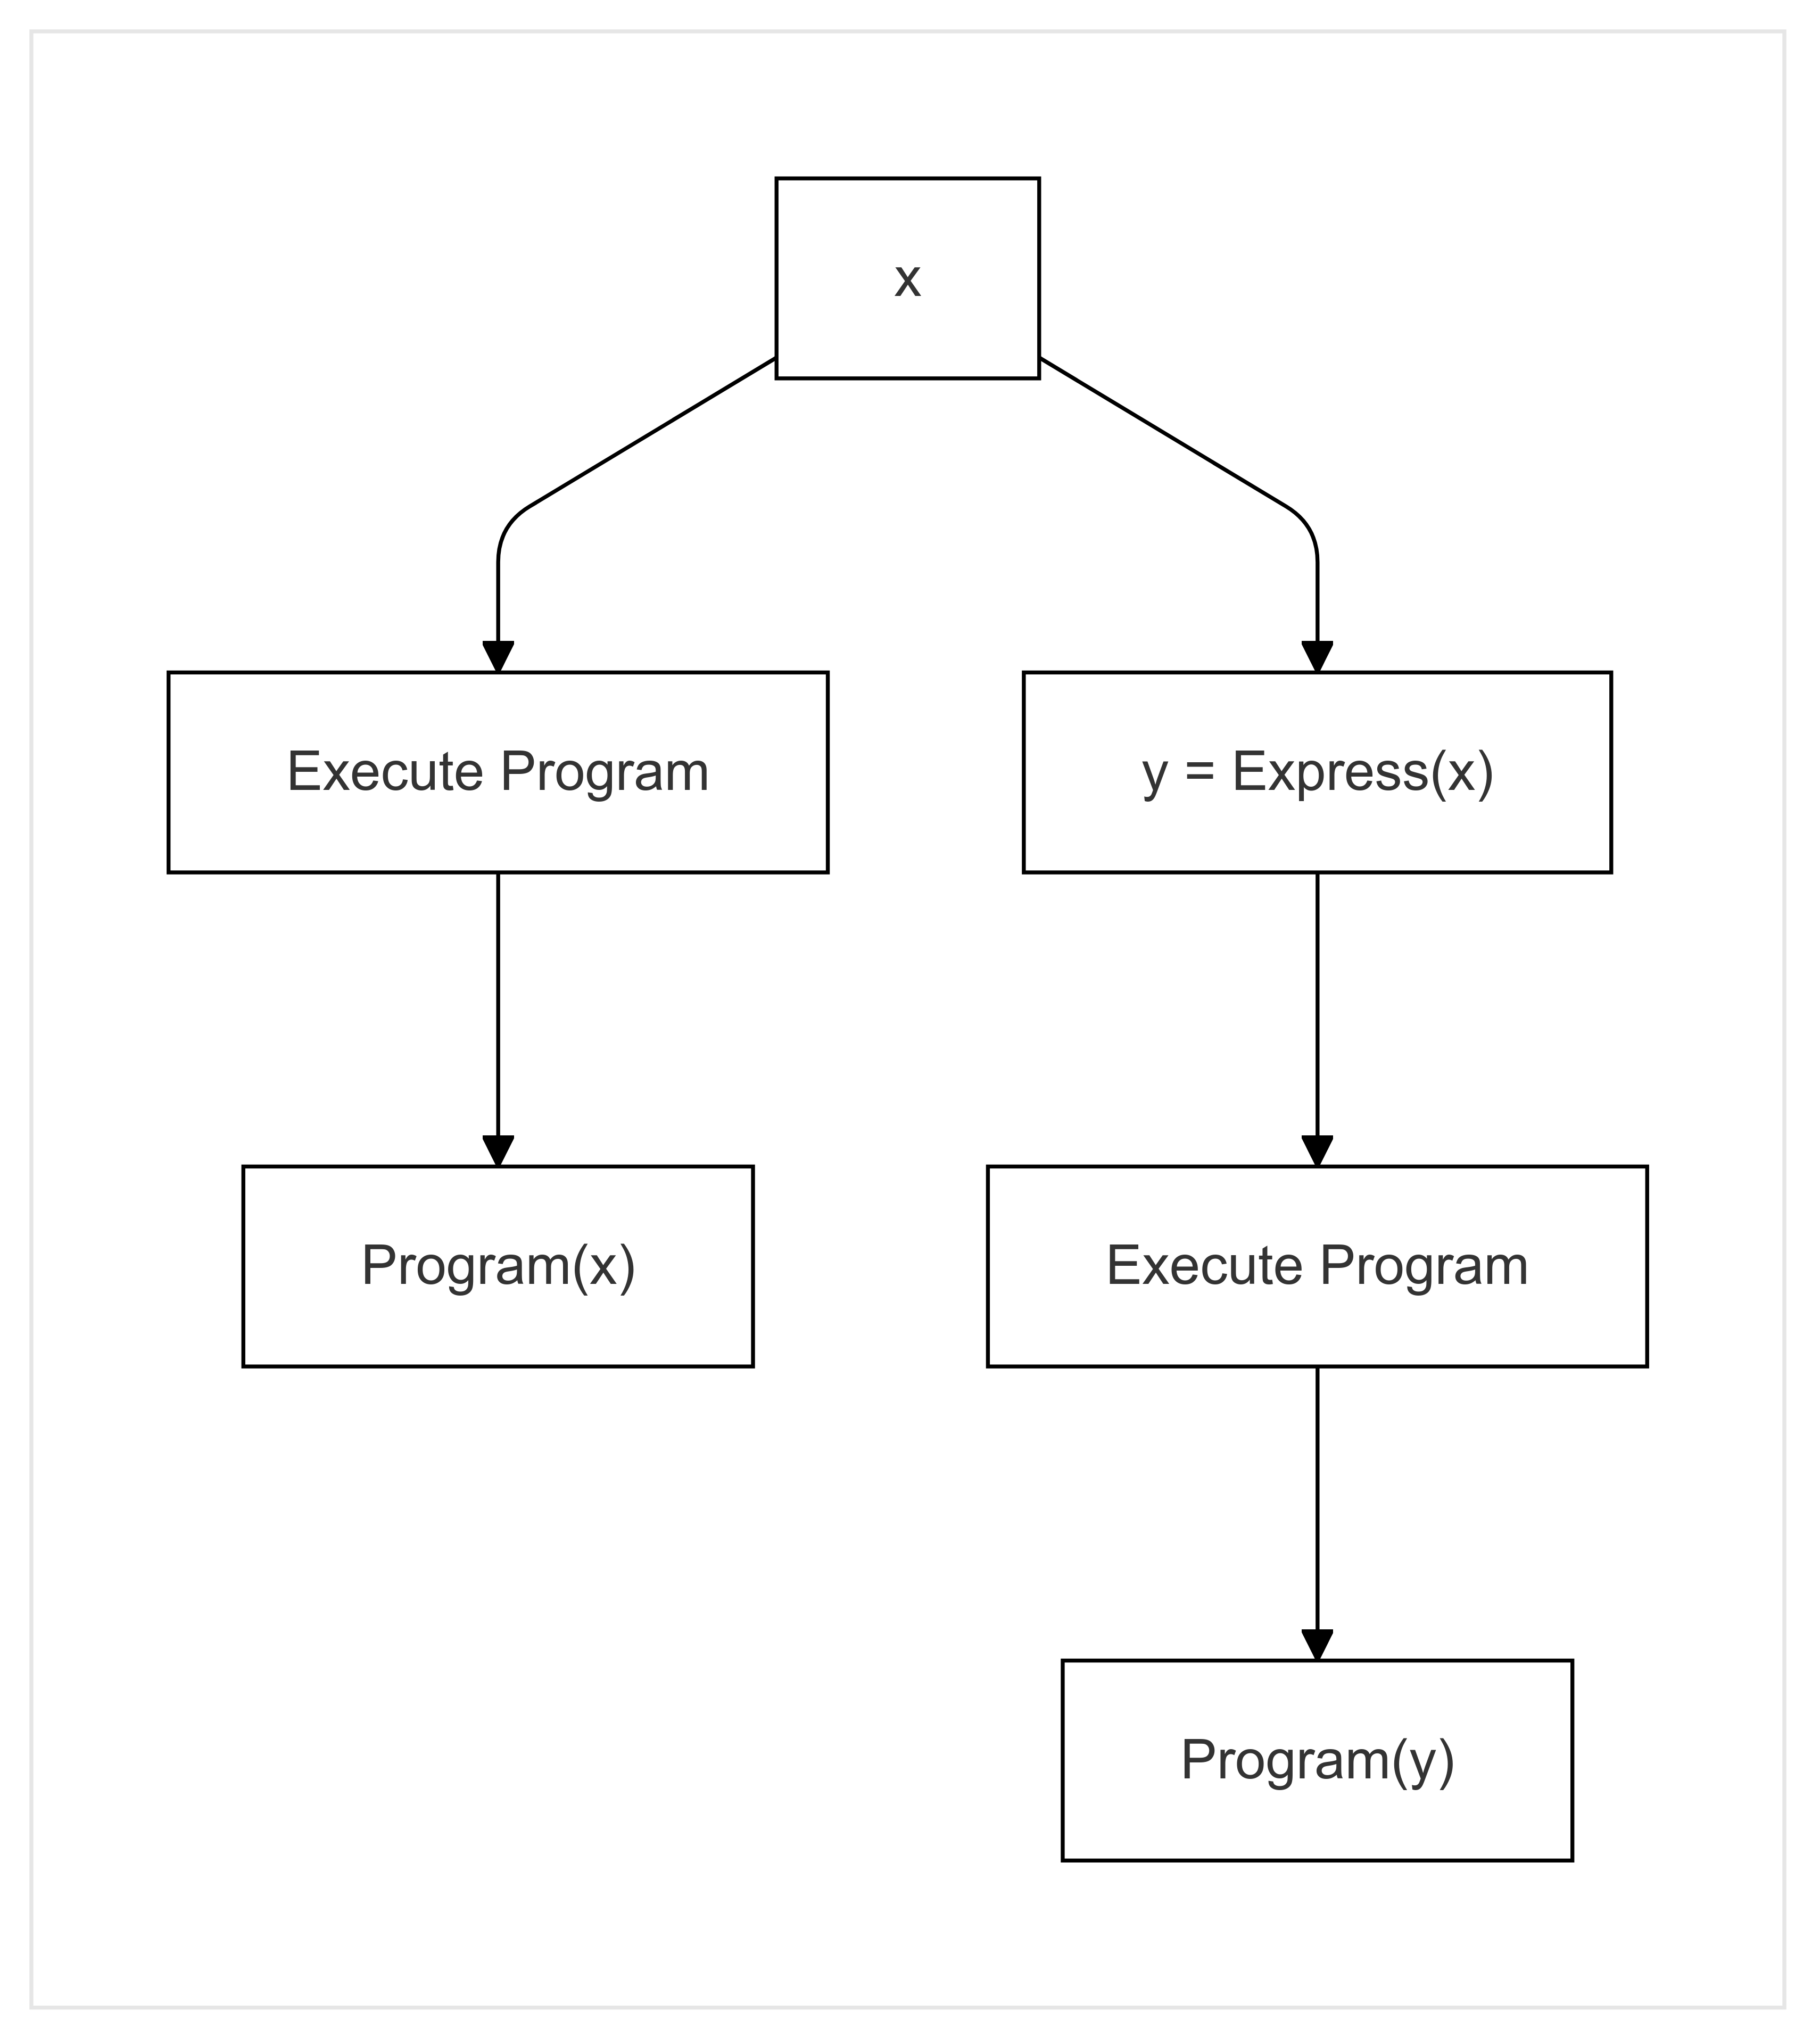
\includegraphics[width=0.7\textwidth]{diagrams/data_div/reexpress.png}
    \caption{Data Reexpression}
    \label{fig:data_rex}
\end{figure}

\subsection{Miscellaneous}
(Name is subject to change.)
This category is dedicated to fault tolerance methods which do not strictly fall into any of the aforementioned categories but are still worth consideration.

\textbf{Framework} can be considered any fault tolerance technique which instead of aiming to directly create fault tolerant software provides a wrapper or tooling to help create fault tolerant software. Benefit of frameworks is the fact that the software developers do not have to concern themselves with fault tolerance, since the overarching framework is responsible for that. Example might be an OS designed to be fault tolerant.

Another interesting example is specialized compiler which embeds fault tolerance into the software during compilation, independently of the actual software's purpose. Example of this approach is \textbf{"Control flow checking by software signature"} published in \cite{994926}.

\section{Motivation for Rust}
One of the main purposes of this thesis is to analyze the suitability of Rust language for the implementation of fault-tolerant software. Historically, C has been the most dominant language in this problem space, but Rust has numerous benefits which make it a strong candidate.

\subsection{Safe by design}
The goal of the Rust language is to eliminate the most common software bugs at the compiler level. An example of this is Rust's \textit{ownership and borrowing model} - a static code analysis done by the compiler \cite{rust_book:ownership}. It ensures memory safety of the program by explicity disallowing references to deallocated values, which prevents null pointer dereferencing, and also prevents race conditions by limiting the access to mutable variables. Rust's ownership model is a complex topic and explaning it in full is not within the scope of this thesis, more information can be found in the offical Rust book.

\subsection{Robust error handling}
Another major benefit of Rust is its approach to error handling. Rust splits errors into two categories: \textit{Unrecoverable} errors immediately terminate the execution of the program using the \textit{panic!()} macro \cite{rust_book:panic}, meaning there is not much to say about them. And \textit{recoverable} errors which are return values of a function using the Result<T, E> enum \cite{rust_book:result}. Using the approach of \textit{error-as-a-value} we can determine if a function executed successfully by simply checking its return value. This can function as a very quick and rudimentary form of fault tolerance, since it can be easily applied to any function.
\newpage
\begin{figure}
\begin{lstlisting}[language=Rust]
fn foo() -> Result<u32, ()> {
    ...
}

fn main() {
    let Ok(res) = foo() else {
        // Function did not execute properly!
    }
}
\end{lstlisting}
\caption{Rust - error as a value}
\label{fig:rust_error}
\end{figure}


\subsection{Macro system}
Rust has a powerful macro system which in essence works as a code pre-processor acting over the abstract syntax tree. Unlike C macros, which only work as direct text replacement, Rust macros allow for arbitrary modification and generation of code before the compilation step. Using Rust macros, various fault tolerance techniques can be easily implmeneted, which would be very tedious to do with a more simple macro system. An example of utilizing macros is highlighted in this very thesis, where a Control Flow Checkign using Signature Streams (CFCSS) technique is implemented using Rust macro system. 

\subsection{Low-level control and C integration}
Rust demonstrates comparable functionality to C when it comes to low-level control - example being the ability to define custom heap allocator or the ability to use in-line assembly from within Rust. Since Rust uses LLVM under the hood, its compiler is able to link against existing C code. This makes for and easy integration with existing C projects making Rust well suited as a higher level extension. This thesis demonstrates the use of Rust with FreeRTOS codebase written in C.

\begin{figure}
\begin{lstlisting}[language=Rust]
unsafe extern "C" {
    fn puts(string: *const c_char, len: usize) -> i32;
}
\end{lstlisting}
\caption{Rust - Using C function within Rust}
\label{fig:rust_extern}
\end{figure}

\newpage

\section{Implementation}



\begin{lstlisting}[language=Rust]
    use rand::seq::SliceRandom;
    use rand::thread_rng;
    
    /_
    Function to process input data, this only works
    if the function does not care about the order of the input.
    _/
    fn process_data(input: &[u64]) -> Result<bool, String> {
    if input[0] == 0 {
    return Err("edge-case".into());
    }
    
        Ok(true)
    
    }
    
    fn main() -> Result<(), String> {
    let mut input: Vec<u64> = vec![0, 1, 2];
    
        // Keep retrying the function until it succeeds
        let output = loop {
            match process_data(&input) {
                Err(error) => {
                    println!("error: {}", error);
    
                    // Reshuffle input
                    input.shuffle(&mut thread_rng());
                }
                Ok(output) => break output,
            }
        };
    
        println!("correct output: {}", output);
    
        Ok(())
    
    }
    \end{lstlisting}

\section{Roadmap}

\begin{enumerate}[label=\arabic*.]
    \item \textbf{Analysis of the problem} - \textit{Done}
    \item \textbf{Research} - \textit{Done}
    \item \textbf{Gathering references} - \textit{Mostly Done}
    \item \textbf{Compile relevant information and research into a document (basis for the thesis)} - \textit{Mostly Done}
    \item \textbf{Add diagrams and code snippets} - \textit{Done}
    \item \textbf{Select fault tolerance techniques to implement} - \textit{Mostly Done}
    \item \textbf{Get FreeRTOS working locally} - \textit{Done}
    \item \textbf{Implement basic application using FreeRTOS} - \textit{Started}
    \item \textbf{Implement fault tolerance application using FreeRTOS} - \textit{Not Started}
\end{enumerate}

\newpage
\printbibliography

\end{document}